\chapter{Multiphysics topology optimization problems}

CHECK COPYRIGHT FOR FIGURES AND REPRINTS

In this chapter we will focus on the effects of multiphysics couplings in nanophotonic devices, reviewing state-of-the-art research, 
highlighting open topology optimization problems, and presenting our contributions to the field.
We will focus on three main classes of multiphysics couplings: thermo-optical, opto-mechanical, and electro-optical systems.
%\begin{figure}[tb]
%    \centering
%    \makebox[\textwidth][c]{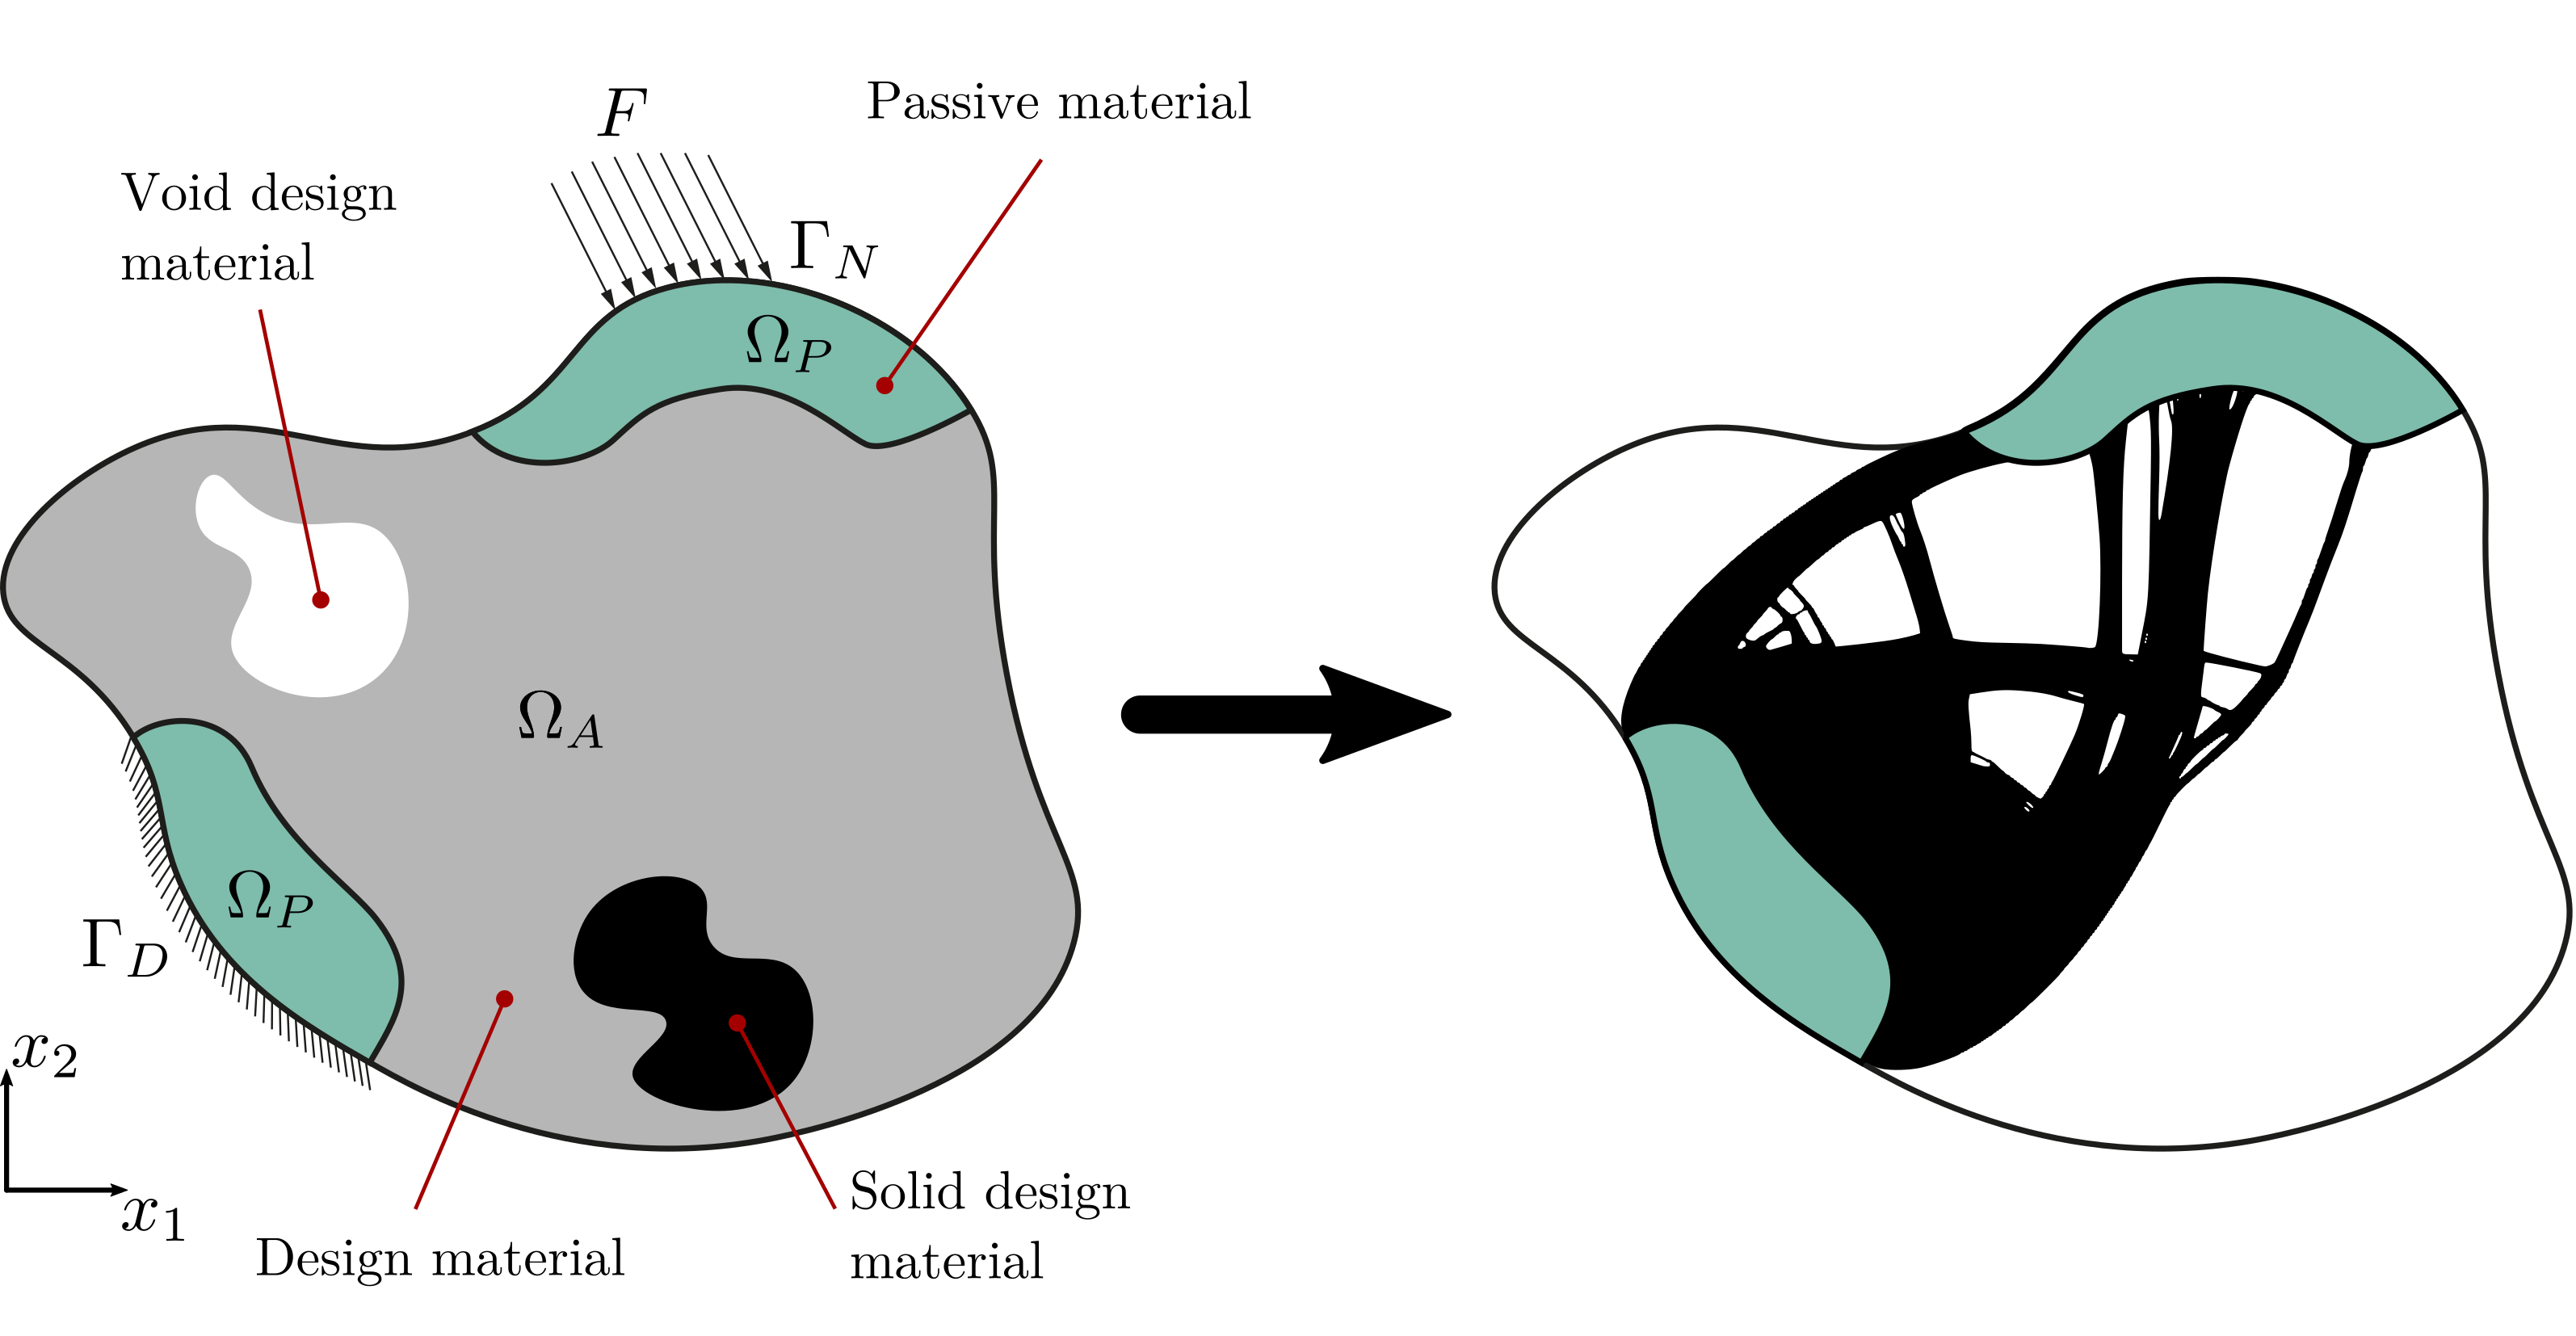
\includegraphics[width=1\imwidth]{figures/simpModel.png}}%
%    \caption{Bla bla bla...}
%    \label{fig:illustateTopOpt}
%\end{figure}


%\begin{equation}
%    (EIu'')'' = q
%\end{equation}


%\begin{figure}[tb]
%    \centering
%    \makebox[\textwidth][c]{\begin{tikzpicture}[remember picture]
    \begin{scope}[xshift=0mm]
        % angle (deg)
        \newcommand\ai{10}
        % line width
        \newcommand\wi{1pt}
        % cell size
        \newcommand\cellsize{3}
        % Rank-$N$ size
        \newcommand\di{0.75}

        % cell
        \draw[gray!10,   fill=gray!10, rotate around={\ai:(0,0)}] (0,0) rectangle (\cellsize,\cellsize) node (rect1) {};
        \draw[black!60, fill=black!60, rotate around={\ai:(0,0)}] (0,0) rectangle (\di,\cellsize);

        % orientation frame
        \draw[black, -stealth, line width=\wi, rotate around={\ai:({\di*cos(\ai) - \cellsize/2*sin(\ai)},{\di*sin(\ai) + \cellsize/2*cos(\ai)})}] ({\di*cos(\ai) - \cellsize/2*sin(\ai)},{\di*sin(\ai) + \cellsize/2*cos(\ai)}) -- ({\di*cos(\ai) - \cellsize/2*sin(\ai) + 0.75},{\di*sin(\ai) + \cellsize/2*cos(\ai)});
        \draw[black, -stealth, line width=\wi, rotate around={\ai:({\di*cos(\ai) - \cellsize/2*sin(\ai)},{\di*sin(\ai) + \cellsize/2*cos(\ai)})}] ({\di*cos(\ai) - \cellsize/2*sin(\ai)},{\di*sin(\ai) + \cellsize/2*cos(\ai)}) -- ({\di*cos(\ai) - \cellsize/2*sin(\ai)},{\di*sin(\ai) + \cellsize/2*cos(\ai) + 0.75});

        % local frame
        \draw[black, -stealth, dashed, line width=\wi] (0,0) -- ({\cellsize + 0.8},0);
        \draw[black, -stealth, dashed, line width=\wi] (0,0) -- (0,{\cellsize + 0.8});

        % ruler
        \draw[black, |-|, line width=\wi, rotate around={\ai:(0,0)}] (0,0) -- (\cellsize,0);
        \draw[black,  -|, line width=\wi, rotate around={\ai:(0,0)}] (0,0) -- (\di,0);

        % arc
        \draw[black, dotted, line width=\wi] (\cellsize,0) arc (0:\ai:\cellsize);

        % annotation
        \draw (\cellsize + 0.7, -0.3) node {$x_1 / \epsilon^3$};
        \draw (-0.5, \cellsize + 0.8) node {$x_2 / \epsilon^3$};
        \draw (\cellsize/2,-0.75) node {Rank-$1$};

        \draw[rotate around={{\ai/2}:(0,0)}] ({\cellsize+0.3},0) node {$\theta_1$};

        \draw[rotate around={{\ai}:(0,0)}] ({\di/2},0.4) node [rotate around={{\ai}:(0,0)}] {$\mu_1$};
        \draw[rotate around={{\ai}:(0,0)}] ({(\cellsize - \di)/2 + \di},0.4) node [rotate around={{\ai}:(0,0)}] {$1-\mu_1$};

        \draw[rotate around={{\ai}:(0,0)}] ({0+0.4},{\cellsize-0.4}) node [rotate around={{\ai}:(0,0)}] {$(+)$};
        \draw[rotate around={{\ai}:(0,0)}] ({\cellsize-0.4},{\cellsize-0.4}) node [rotate around={{\ai}:(0,0)}] {$(-)$};
        \coordinate (A) at (rect1.north);


        \draw[rotate around={\ai:({\di*cos(\ai) - \cellsize/2*sin(\ai)},{\di*sin(\ai) + \cellsize/2*cos(\ai)})}] ({\di*cos(\ai) - \cellsize/2*sin(\ai)+1} , {\di*sin(\ai) + \cellsize/2*cos(\ai) + 0.2}) node {$\mathbf{n}_1$};
        \draw[rotate around={\ai:({\di*cos(\ai) - \cellsize/2*sin(\ai)},{\di*sin(\ai) + \cellsize/2*cos(\ai)})}] ({\di*cos(\ai) - \cellsize/2*sin(\ai) + 0.3} , {\di*sin(\ai) + \cellsize/2*cos(\ai) + 1}) node {$\mathbf{m}_1$};



    \end{scope}
    \begin{scope}[xshift=45mm]
        % angle (deg)
        \newcommand\ai{15}
        % line width
        \newcommand\wi{1pt}
        % cell size
        \newcommand\cellsize{3}
        % Rank-$N$ size
        \newcommand\di{0.6}

        % cell
        \draw[gray!40,   fill=gray!40, rotate around={\ai:(0,0)}] (0,0) rectangle (\cellsize,\cellsize) node (rect2) {};
        \draw[black!60, fill=black!60, rotate around={\ai:(0,0)}] (0,0) rectangle (\di,\cellsize);

        % orientation frame
        \draw[black, -stealth, line width=\wi, rotate around={\ai:({\di*cos(\ai) - \cellsize/2*sin(\ai)},{\di*sin(\ai) + \cellsize/2*cos(\ai)})}] ({\di*cos(\ai) - \cellsize/2*sin(\ai)},{\di*sin(\ai) + \cellsize/2*cos(\ai)}) -- ({\di*cos(\ai) - \cellsize/2*sin(\ai) + 0.75},{\di*sin(\ai) + \cellsize/2*cos(\ai)});
        \draw[black, -stealth, line width=\wi, rotate around={\ai:({\di*cos(\ai) - \cellsize/2*sin(\ai)},{\di*sin(\ai) + \cellsize/2*cos(\ai)})}] ({\di*cos(\ai) - \cellsize/2*sin(\ai)},{\di*sin(\ai) + \cellsize/2*cos(\ai)}) -- ({\di*cos(\ai) - \cellsize/2*sin(\ai)},{\di*sin(\ai) + \cellsize/2*cos(\ai) + 0.75});

        % local frame
        \draw[black, -stealth, dashed, line width=\wi] (0,0) -- ({\cellsize + 0.8},0);
        \draw[black, -stealth, dashed, line width=\wi] (0,0) -- (0,{\cellsize + 0.8});

        % ruler
        \draw[black, |-|, line width=\wi, rotate around={\ai:(0,0)}] (0,0) -- (\cellsize,0);
        \draw[black,  -|, line width=\wi, rotate around={\ai:(0,0)}] (0,0) -- (\di,0);

        % arc
        \draw[black, dotted, line width=\wi] (\cellsize,0) arc (0:\ai:\cellsize);

        % annotation
        \draw (\cellsize + 0.7, -0.3) node {$x_1 / \epsilon^2$};
        \draw (-0.5, \cellsize + 0.8) node {$x_2 / \epsilon^2$};
        \draw (\cellsize/2,-0.75) node {Rank-$2$};

        \draw[rotate around={{\ai/2}:(0,0)}] ({\cellsize+0.3},0) node {$\theta_2 + \pi/4$};

        \draw[rotate around={{\ai}:(0,0)}] ({\di/2},0.4) node [rotate around={{\ai}:(0,0)}] {$\mu_2$};
        \draw[rotate around={{\ai}:(0,0)}] ({(\cellsize - \di)/2 + \di},0.4) node [rotate around={{\ai}:(0,0)}] {$1-\mu_2$};

        \draw[rotate around={{\ai}:(0,0)}] ({0+0.4},{\cellsize-0.4}) node [rotate around={{\ai}:(0,0)}] {$(+)$};
        \draw[rotate around={{\ai}:(0,0)}] ({\cellsize-0.9},{\cellsize-0.4}) node [rotate around={{\ai}:(0,0)}] (B) {$(\text{Rank-1})$};
        \coordinate (B2) at (rect2.north);


        \draw[rotate around={\ai:({\di*cos(\ai) - \cellsize/2*sin(\ai)},{\di*sin(\ai) + \cellsize/2*cos(\ai)})}] ({\di*cos(\ai) - \cellsize/2*sin(\ai)+1} , {\di*sin(\ai) + \cellsize/2*cos(\ai) + 0.2}) node {$\mathbf{n}_2$};
        \draw[rotate around={\ai:({\di*cos(\ai) - \cellsize/2*sin(\ai)},{\di*sin(\ai) + \cellsize/2*cos(\ai)})}] ({\di*cos(\ai) - \cellsize/2*sin(\ai) + 0.3} , {\di*sin(\ai) + \cellsize/2*cos(\ai) + 1}) node {$\mathbf{m}_2$};


    \end{scope}
    \begin{scope}[xshift=90mm]
        % angle (deg)
        \newcommand\ai{20}
        % line width
        \newcommand\wi{1pt}
        % cell size
        \newcommand\cellsize{3}
        % Rank-$N$ size
        \newcommand\di{1.0}

        % cell
        \draw[gray!60,   fill=gray!60, rotate around={\ai:(0,0)}] (0,0) rectangle (\cellsize,\cellsize);
        \draw[black!60, fill=black!60, rotate around={\ai:(0,0)}] (0,0) rectangle (\di,\cellsize);

        % orientation frame
        \draw[black, -stealth, line width=\wi, rotate around={\ai:({\di*cos(\ai) - \cellsize/2*sin(\ai)},{\di*sin(\ai) + \cellsize/2*cos(\ai)})}] ({\di*cos(\ai) - \cellsize/2*sin(\ai)},{\di*sin(\ai) + \cellsize/2*cos(\ai)}) -- ({\di*cos(\ai) - \cellsize/2*sin(\ai) + 0.75},{\di*sin(\ai) + \cellsize/2*cos(\ai)});
        \draw[black, -stealth, line width=\wi, rotate around={\ai:({\di*cos(\ai) - \cellsize/2*sin(\ai)},{\di*sin(\ai) + \cellsize/2*cos(\ai)})}] ({\di*cos(\ai) - \cellsize/2*sin(\ai)},{\di*sin(\ai) + \cellsize/2*cos(\ai)}) -- ({\di*cos(\ai) - \cellsize/2*sin(\ai)},{\di*sin(\ai) + \cellsize/2*cos(\ai) + 0.75});

        % local frame
        \draw[black, -stealth, dashed, line width=\wi] (0,0) -- ({\cellsize + 0.8},0);
        \draw[black, -stealth, dashed, line width=\wi] (0,0) -- (0,{\cellsize + 0.8});

        % ruler
        \draw[black, |-|, line width=\wi, rotate around={\ai:(0,0)}] (0,0) -- (\cellsize,0);
        \draw[black,  -|, line width=\wi, rotate around={\ai:(0,0)}] (0,0) -- (\di,0);

        % arc
        \draw[black, dotted, line width=\wi] (\cellsize,0) arc (0:\ai:\cellsize);

        % annotation
        \draw (\cellsize + 0.7, -0.3) node {$x_1 / \epsilon$};
        \draw (-0.5, \cellsize + 0.8) node {$x_2 / \epsilon$};
        \draw (\cellsize/2,-0.75) node {Rank-$3$};

        \draw[rotate around={{\ai/2}:(0,0)}] ({\cellsize+0.3},0) node {$\theta_3 - \pi/2$};

        \draw[rotate around={{\ai}:(0,0)}] ({\di/2},0.4) node [rotate around={{\ai}:(0,0)}] {$\mu_3$};
        \draw[rotate around={{\ai}:(0,0)}] ({(\cellsize - \di)/2 + \di},0.4) node [rotate around={{\ai}:(0,0)}] {$1-\mu_3$};

        \draw[rotate around={{\ai}:(0,0)}] ({0+0.4},{\cellsize-0.4}) node [rotate around={{\ai}:(0,0)}] {$(+)$};
        \draw[rotate around={{\ai}:(0,0)}] ({\cellsize-0.9},{\cellsize-0.4}) node [rotate around={{\ai}:(0,0)}] (C) {$(\text{Rank-2})$};


        \draw[rotate around={\ai:({\di*cos(\ai) - \cellsize/2*sin(\ai)},{\di*sin(\ai) + \cellsize/2*cos(\ai)})}] ({\di*cos(\ai) - \cellsize/2*sin(\ai)+1} , {\di*sin(\ai) + \cellsize/2*cos(\ai) + 0.2}) node {$\mathbf{n}_3$};
        \draw[rotate around={\ai:({\di*cos(\ai) - \cellsize/2*sin(\ai)},{\di*sin(\ai) + \cellsize/2*cos(\ai)})}] ({\di*cos(\ai) - \cellsize/2*sin(\ai) + 0.3} , {\di*sin(\ai) + \cellsize/2*cos(\ai) + 1}) node {$\mathbf{m}_3$};

    \end{scope}
    \path[-latex,black,thick] (A) edge [bend left=50] (B);
    \path[-latex,black,thick] (B2) edge [bend left=50] (C);
\end{tikzpicture}}%
%    \caption{Bla bla bla...}
%    \label{fig:Rank}
%\end{figure}

%\section{Coupled optical systems}

%TODO: Include if we end up doing the Green's function study.

% Make a connection to the Green's function formalism and derive system of coupled equations.

\section{Thermo-optical systems~\cite{ownpub0}}\label{sec:thermo_optical}

Thermo-optical systems exploit the interplay between the temperature and electromagnetic fields to enable active control over optical properties. 
The main mechanism behind this coupling is the thermo-optic effect, 
in which the refractive index of a material changes as a function of temperature. 
This effect plays a central role in many integrated photonics application; such as,
 optical phase shifters~\cite{TOPS_1, TOPS_2, TOPS_3}, reconfigurable photonic circuits~\cite{program, PIC}, and thermally tunable switches~\cite{switch, switch_2} and filters~\cite{filter}.

 Despite its wide usage, optimizing thermo-optical devices remains challenging due to the intricate coupling 
 between thermal and optical physics. Topology optimization offers a systematic design optimization solution, with application examples in
  thermo-optical phase shifters~\cite{TOPS_heat, ownpub0}, optical mirror-like thermo-mechanical structures~\cite{opt_perf}, and
strcutural integrity constraints~\cite{structural_heat}, among others.

In the following sections, we summarize how to model and optimize thermo-optic systems, 
with special focus on our research contribution~\cite{ownpub0}, which to the best of our knowledge,
extends the state-of-the art uncoupled and single-physics thermo-optic topology optimization frameworks by, for the first time, considering 
the coupled physical problem.

\subsection*{The thermo-optic effect: coupling heat-transfer with optics}

To model the coupled thermo-optical topology optimization problem, we combine the governing equation of the optical model [\eqref{eq:wave_eq}]
with a heat transfer model. The simplest heat trasfer model is the steady-state heat equation, which describes the
heat transfer in a medium due to conduction and heat sources. The heat equation is given by
\begin{equation}\label{eq:heat}
    -\nabla \cdot (\kappa \nabla T) = Q
\end{equation}
where $T$ is the temperature, $\kappa$ is the thermal conductivity, and $Q$ is a volumetric heat source. Note that this equation can be
extended by consider convection and radiation effects, which may be important in some thermo-optical systems (see the boundary conditions
in~\cite{ownpub0}).

This temperature can be coupled to the optical response via the therm-optic coefficient (TOC), which links the temperature field
with the refractive index of the material, typically approximated with the linear relation\footnote{Large temperature gradients may lead to nonlinear effects, requiring higher order terms.}
\begin{equation}
n(\mathbf{r}) = n_0 + \text{TOC} \cdot \left[T(\mathbf{r}) - T_0\right],
\end{equation}
where $n_0$ and $T_0$ are the reference (unheated) refractive index and reference temperature, respectively. Thus, to solve a problem coupled throught the TOC, one first solves the heat equation
to determine the temperature, which can be used to determine
the spatially varying refractive index, which is then used in \eqref{eq:wave_eq} to determine the optical field. In topology optimization
problems, one uses an additional material interpolation to link the physical field with the design-dependent conductivity, or heat source.

\subsection*{Thermo-optical phase-shifter topology optimization~\cite{ownpub0}}

Among the many applications that utilize the thermo-optic coefficient, we find integrated photonic circuit components, which rely on the large 
TOC of silicon ($\text{TOC} \approx 1.8 \cdot 10^{-4}\, \text{K}^{-1}$) at room-temperature ($\approx300$ K) and telecom wavelength 
($\lambda=1.55$ \textmu m)~\cite{thermo-optic-coef}. One of those components is the thermo-optical phase shifter, which, as shown in \figref{fig:thermo_opt},
uses a heating device to locally modify the refractive index of a waveguide structure to induce a phase shift ($\Delta \Phi$) in the propagating optical mode
\begin{equation*}
\Delta \Phi = \frac{2\pi L}{\lambda} \Delta n_\text{eff},
\end{equation*}
where $L$ is the device length and $\Delta n_\text{eff} = n_\text{eff, heated} - n_\text{eff, unheated}$ is the change of the effective index of the waveguide. 
In order to calculate the phase-shift one thus needs to find the effective index of an optical mode, which can be done by 
using the finite-element formulation for two-dimensional waveguide cross-sections~\cite{jin}:
\begin{equation}\label{eq:wg_eq}
    \left[\begin{array}{cc}
    A_{\text{tt}}(\varepsilon,k) & 0 \\
    0 & 0
    \end{array}\right]
    \left\{\begin{array}{l}
    E_{\text{t}} \\
    E_z
    \end{array}\right\}
    = -k_z^2
    \left[\begin{array}{cc}
    B_{\text{tt}} & B_{\text{t} z} \\
    B_{z \text{t}} & B_{z z}(\varepsilon,k)
    \end{array}\right]
    \left\{\begin{array}{c}
    E_{\text{t}} \\
    E_z
    \end{array}\right\},
    \end{equation}
where $E_{\text{t}}$ and $E_z$ are the transverse and longitudinal electric field components, $k_z$ is the propagation constant of the optical mode, and $A_{tt}, B_{tt},
B_{zt}$ and $B_{tz}$ are matrices that can be assembled using the interpolation functions. Following~\cite{jin}, we use first-order Nédélec elements for in-plane components and 
second-order Lagrange elements for out-of-plane components\footnote{Lagrange elements must be one order higher than edge elements to properly represent gradients or curls.}. 
Solving the generalized eigenvalue problem in \eqref{eq:wg_eq} yields waveguide modes ($E_t$, $E_z$) and propagation constants ($k_z$). The propagation constant can be rewritten into the effective index $n_\text{eff} = k_z / k$,
 where the real part is a measure of the mode overlap with the refractive index distribution, and the imaginary part ($\Im\{n_\text{eff}\}$) quantifies optical losses. 

Recent progress in waveguide design by U.D. Dave and M. Lipson~\cite{lipson}, proposed the use of PT-symmetry breaking waveguides as good canditates for
thermo-optical phase shifters, since they can minimize optical losses near (lossy) metallic heaters. To understand this phenomenon we solve the generalized
eigenvalue problem in \eqref{eq:wg_eq} for a waveguide where half of the core is lossy (characterized by $\Im\{n\}>0$).  As loss increases, the fundamental mode becomes more lossy until reaching an (exceptional) 
point where it bifurcates into high- and low-loss modes. Surprisingly, further increasing $\Im\{n\}$ counter-intuitively reduces the loss of the low-loss mode. This effect is particularly useful in the design of
thermo-optical waveguide devices, since it enables to position a lossy metallic heater in direct contact with the waveguide core, while the mode is still able to propagate with low losses.

\begin{figure}[tb]
    \centering
    \makebox[\textwidth][c]{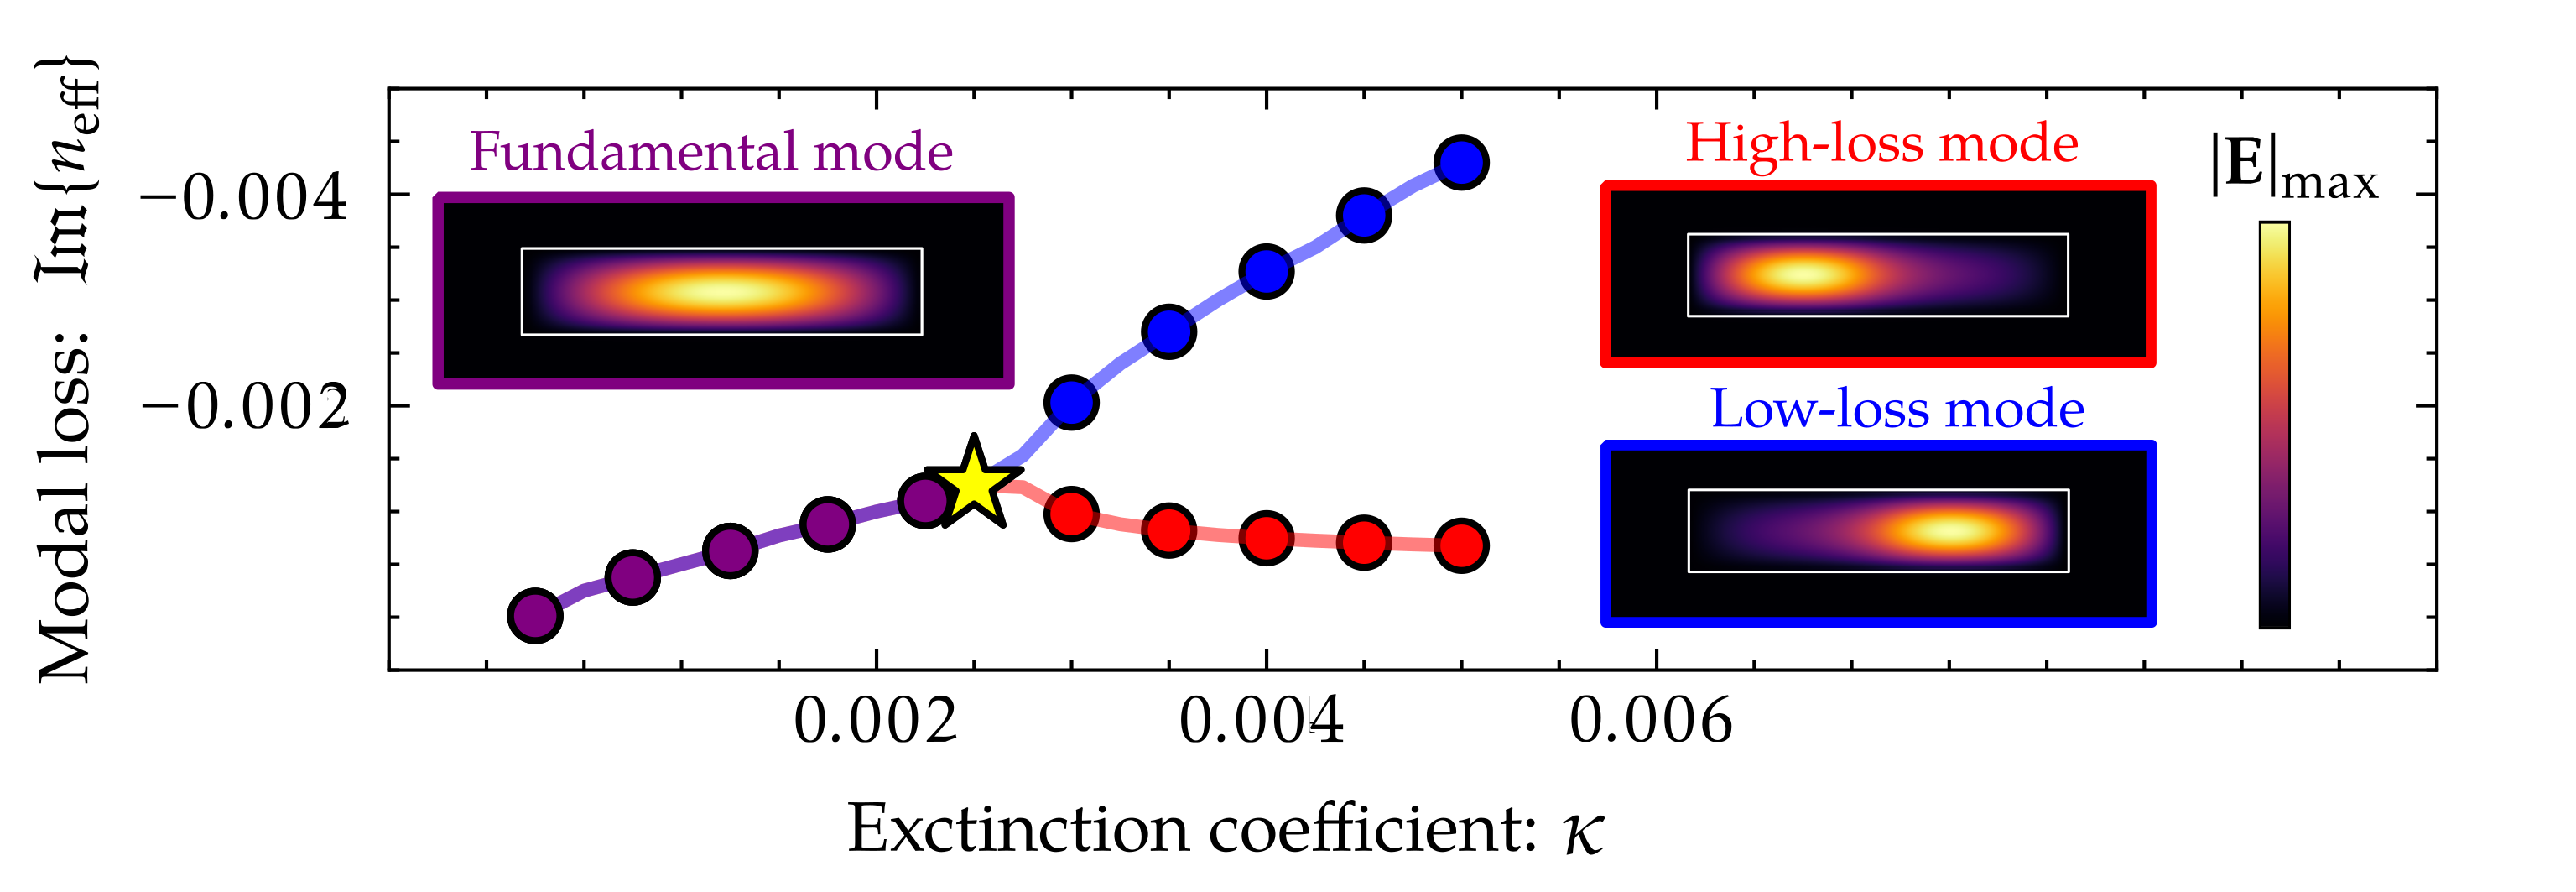
\includegraphics{figures/TOPS_pt.png}}%%
    \caption{Parity-time symmetry breaking and interpretation of losses of propagating modes. Make this figure look better.}
    \label{fig:thermo_opt}
\end{figure}

Inspired by PT-symmetry breaking waveguides, in~\cite{ownpub0} we use topology optimization to have good heat conduction and low optical loss in thermo-optical phase shifters.
The optimization problem considers a waveguide cross-section with a metallic heater, and seeks to minimize optical loss in an optical waveguide for both heated and 
unheated configurations. Unlike the eigenvalue-based approach in~\cite{lipson}, in this work we evaluate losses by solving a linear system of equations where we excite the waveguide 
and calculate the excited mode's 
amplitude. As illustrated in \figref{fig:thermo_opt}, maximizing the mode amplitude, is equivalent minimizing the width of the effective 
index resonance, and thus the loss of the mode. Based on this insight, we formulate the optimization problem, where we design the metalic heater around the waveguide, by using a worst-case maximization 
of the electric-field intensity at two effective indices corresponding to heated and unheated 
waveguide configurations. To integrate the heat problem into the topology optimization framework we use a linear material interpolation 
for the conductivity and an interpolation for the heat source
\begin{equation}
    Q(\hat{\rho})=P_{\text{in}} \frac{\hat{\rho}^p}{L a_e \sum_j \hat{\rho}_j}\,,
\end{equation}
where $P_\text{in}$ is the input power in the heater, $p=3$ is a penalization factor, and $a_e$ is the area of the element. With these interpolations we can solve a design-dependent
heat problem which then is fed into the optical problem to calculate the amplitude of the unheated and heated modes. To solve the inverse design
problem we derive a coupled adjoint sensitivity analysis, as further detailed in~\cite{ownpub0}, enabling the use of gradient-based optimization. CHECK AND
MENTION IF THE OPTIMIZE DEVICES RELY ON THE PT-SYMMETRY BREAKING EFFECT. COMMENT ON IT.

Using this framework we find the results in \figref{fig:thermo_res}, where we depict the optimized waveguide cross-section with a metallic heater, which is able to homogeneously heat the waveguide core,
allowing the same low-loss mode to propagate in both the heated and unheated scenarios. Moreover, several extensions of the topology optimization problem are considered for varying volume constraints, optical power, and including fabrication constraints (e.g. minimum lengthscales, and layered 
litography processes). SAY HOW MucH IMPROVEMENT WE GOT!

\begin{figure}[tb]
    \centering
    \makebox[\textwidth][c]{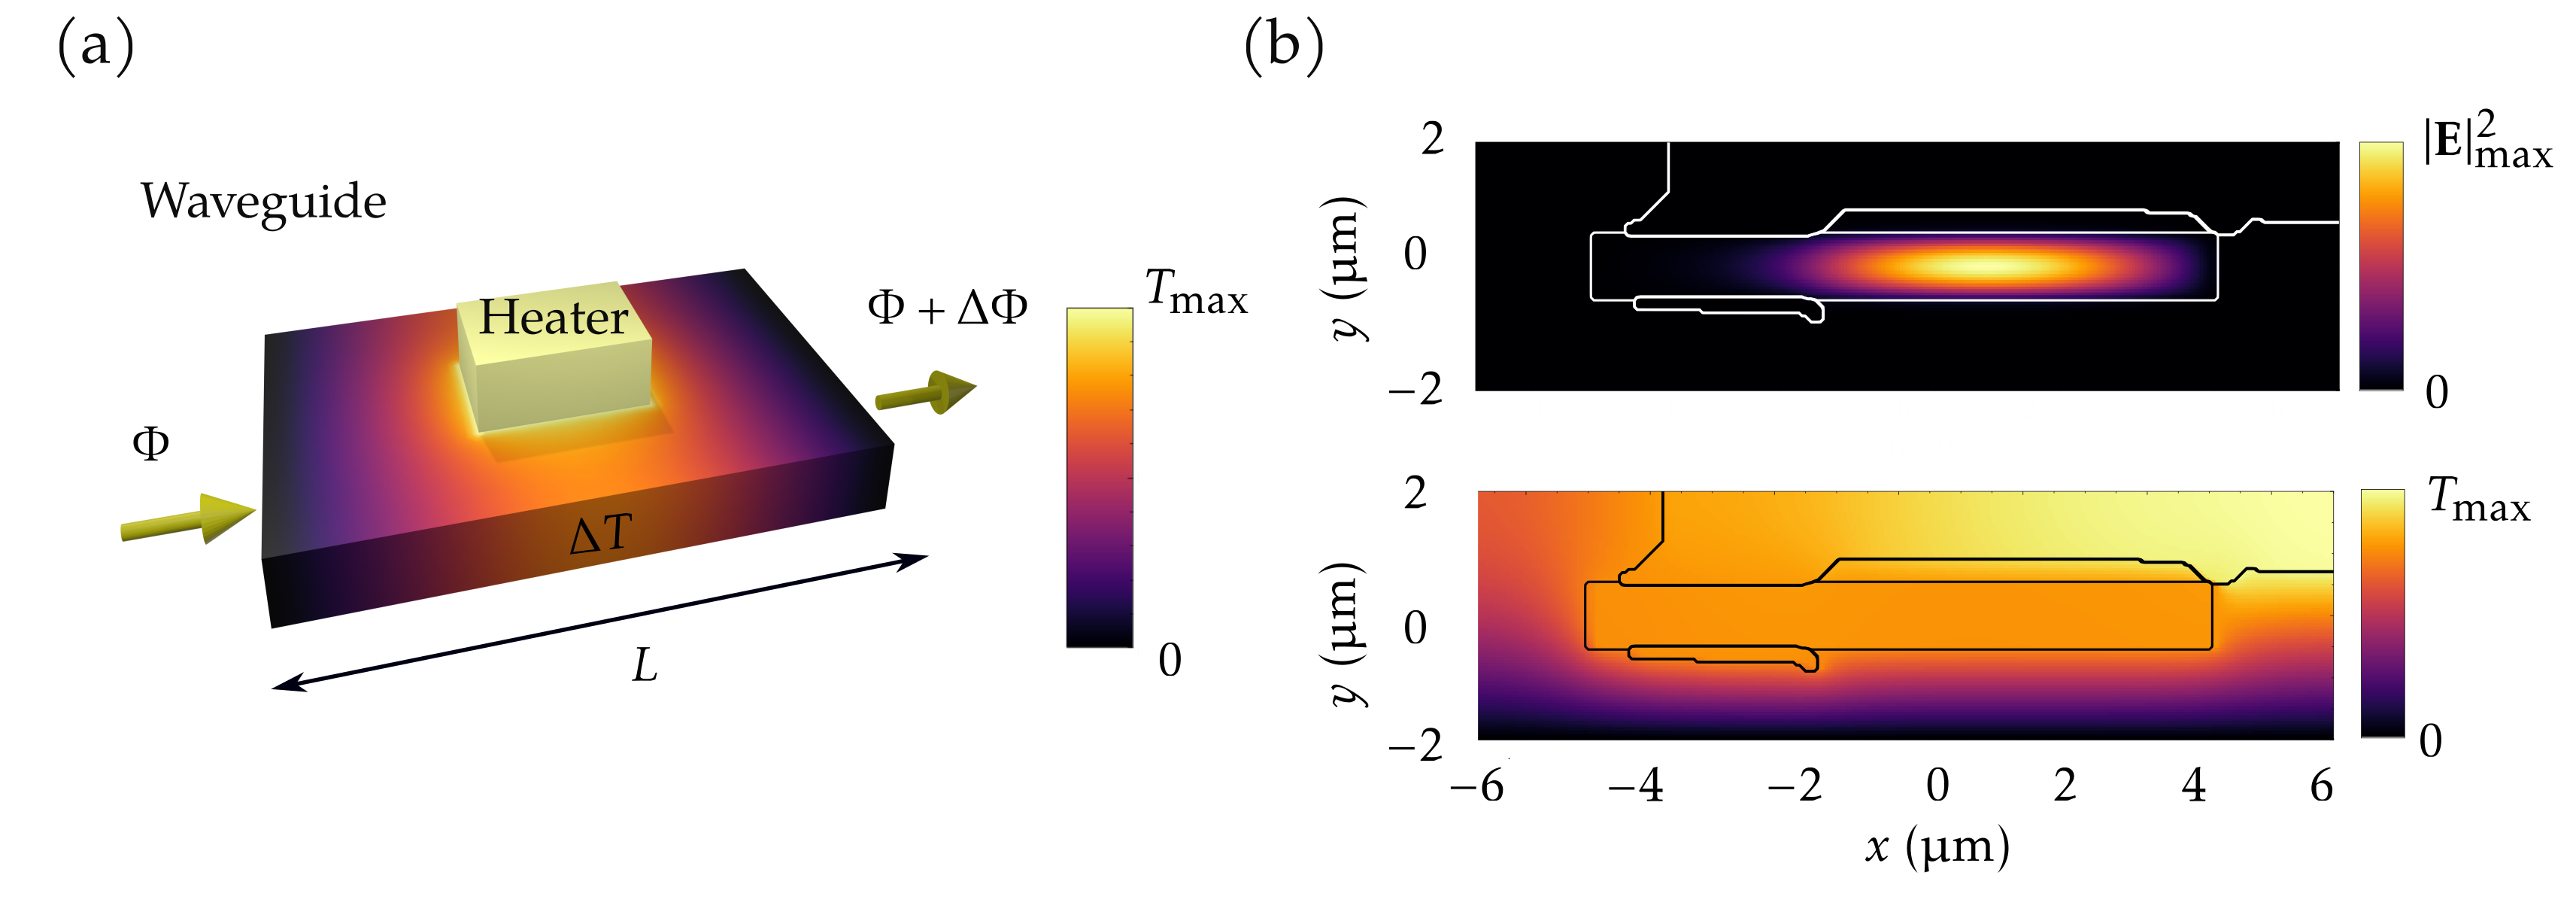
\includegraphics{figures/TOPS_results.png}}%%
    \caption{Topology optimization of thermo-optical phase-shifters. (a) Phase-shifting mechanism, where a heater changes the temperature in the waveguide $\Delta T$, which for a length $L$ creates a phase-shift
    $\Delta \Phi$. (b) Thermal and optical response of the topology optimized device. Adapted with permission from~\cite{ownpub0} \copyright Optical Society of America.}
    \label{fig:thermo_res}
\end{figure}

The framework laid out in our work~\cite{ownpub0} opens up the avenue for the study and optimization to weakly coupled topology optimization problems. For example, for the design of phase-shifters and thermo-optical modulators, it should be straightforward to extend this
formalism to three dimensional system, where one could account for insertion/coupling losses of the integrated photonic circuits. Another example could be the to use multi-material topology optimization, to design not-only the heating
device, but also the optical waveguide. Finally, this formalism could be applied to design completely different devices, such as re-configurable photonic systems that might be modulated by an external heat source, or thermo-optical
switches based on optical cavities~\cite{switch, switch_2}, where the change in refractive index shifts the cavity in- or out-of-resonance.

SAY THAT CONDUCTION AND ELECTROSTATICS ARE SIMILAR CITE POCKELS PAPER AND TALK ABOUT ELECTRO-OPTICAL MODULATION!

\subsection*{Towards strong coupling: heat dissipation in optics}

In the strong coupling regime, the optical response will modify the thermal response, and vice versa.
For example, optical absorption can lead to significant local heating, altering the refractive index and modifying the optical field. 
This mutual dependence requires strongly a coupled treatment of the heat and optical problems, 
which can be accounted for by modeling the optical absorption with an electric field dependent volumetric heat source~\cite{plasm_heat_source}
\[
Q(\mathbf{r}) = \frac{1}{2} \omega \varepsilon_0 \operatorname{Im}[\varepsilon(\mathbf{r})] |\mathbf{E}(\mathbf{r})|^2,
\]
where the material losses ($\Im[\varepsilon]$) convert the electromagnetic energy into heat. 
This expression is particularly important in metal nanostructures, where plasmonic resonances can lead to localized temperature increases~\cite{plasm_heat_source}, or in 
high-intensity photonics where even low absorption materials can generate significant heat~\cite{thermal_nl, high_I_T}. Moreover, the thermo-optical feedback can give rise to nonlinear effects, such as self-focusing~\cite{thermal_nl}. As a matter of fact, if we still consider a linear
thermal response and thermo-optico coefficient,
the nonlinearity has the form of a Kerr-type nonlinearity ($\Delta n \propto \vert \mathbf{E} \vert^2$). Accouting and modeling
these effects could open up the avenue for the inverse design of novel nonlinear thermophotonic devices, with potential applications
in integrated nonlinear photonics~\cite{nl_photonics}, metasurfaces~\cite{nl_meta} and plasmonics~\cite{novotny}.


\subsection*{Heat transfer as an auxiliary connectivity constraint}

Lastly, it is worthwile mentioning that the heat equation can be used as an auxiliary equation to enforce connectivity
and structural integrit in topology optimization problems~\cite{vanessa, structural_heat}, which is employed in several of our
works~\cite{ownpub1,ownpub2}. 

This method, introduced in~\cite{li_structural_2016}, is known as the Virtual Temperature
Method (VTM). The core idea of the VTM is to simulate a heat transfer problem on an auxiliary thermal field, where the design 
domain is treated as a heat source and a thermally conductive material, while void regions are modeled as an
insulating material, and a Dirichlet boundary condition ($T = 0$) is imposed on the boundaries where connectivity is required. When 
solving the steady-state heat equation [\eqref{eq:heat}], regions that are disconnected from the boundary 
cannot dissipate heat and therefore attain elevated temperatures. By applying a threshold criterion such as $T < T_\text{thresh}$, disconnected islands in the design can be 
detected and penalized. For instance, in our works~\cite{ownpub1,ownpub2} we compute a measure of the total virtual temperature
by integrating the temperature field over the design domain, and add it as a constraint in the optimization problem:
$\int_{\Omega_D} T \d \Omega \leq \epsilon_C$, where $\Omega_D$ is the design domain and $\epsilon_c$ is sufficiently small constant. This ensures that the final design remains physically connected to the required 
boundaries. 


Note that by appropriately selecting the connecting boundaries it is possible to use the VTM to enforce
structural integrity of the designs~\cite{structural_heat}, although this can also be ensured by solving an auxiliary
mechanical problem~\cite{structural_integrity}. For a more robust connectivity constraint formulation with less parameter tuning (e.g. material conductivies) we refer the reader to the Nonlinear 
Virtual Temperature Method (NVTM)~\cite{nvtm}, and for further details on connectivity constraints we refer the reader to the review 
article by Cool et al.~\cite{vanessa}.

\section{Opto-mechanical systems~\cite{ownpub1,ownpub2,ownpub3}}

Optomechanics, the study of the interaction between light and mechanical motion, is at the heart of state-of-the-art technologies, such as 
optical trapping~\cite{ashkin_acceleration_1970, moffitt_recent_2008} and cooling~\cite{cooling}, quantum information processing~\cite{Andrews_2014, Xi_2025}
, light sails~\cite{lightsail, lightsail1}, and high-precision metrology and sensing~\cite{sensing, weakforce, Li:18, Mason_2019}.

The most basic description of this interaction is given by the Lorentz force, which governs how moving charges respond to electric and magnetic fields:
\begin{equation}\label{eq:lorentz_f}
    \mathbf{\bm{\mathcal{F}}}(\mathbf{r},t) = q \left[ \bm{\mathcal{E}}(\mathbf{r},t) + \mathbf{v}(t) \times \bm{\mathcal{B}}(\mathbf{r},t) \right]\,,
\end{equation}
where $q$ is the charge and $\mathbf{v}$ is the velocity of the particle. This force can be generalized to describe more complex systems,
such as the the force between two current-carrying 
wires (Ampere's force law), and the electromotive force, which is at the core of many techologies, such as induction motors or generators.
In optomechanical systems, shaping the distribution and magnitude of these forces at the micro- and nanoscale is crucial for controlling mechanical motion with light. 
However, designing structures that can efficiently harness and manipulate these interactions often requires navigating highly complex
 parameter spaces and trade-offs between optical, mechanical, and material constraints.

To achieve such precise control, topology optimization has emerged as a a useful design technique enhance or tailor optomechanical interactions.
Recent advances include the design of coupling between optical and elastic
 waves~\cite{photo_topopt}, optical systems with nonlinear deformations~\cite{def_wg}, high-$Q$ optomechanical membranes~\cite{highQ1, fengwen, aragon1},
light sail structures~\cite{lightsail_topopt, lightsail_topopt1},
on-chip optical trapping devices~\cite{ownpub1}, particle design and manipulation~\cite{ownpub2, particle_opt},
and structural integrity constraint formulations~\cite{structural_integrity}
 among others.

 In the following subsections, we highlight our contributions to the field and review how to model optomechanical interactions in three distinct regimes: a general treatment based on the Maxwell stress tensor~\cite{ownpub2}; 
 the dipole approximation for small particles~\cite{ownpub1, ownpub3}; and strongly coupled systems where optical forces can induce significant mechanical deformations.
\subsection*{Optical forces via the Maxwell Stress Tensor formalism~\cite{ownpub3}}

In the most-general case, the optical force can be calculated using the Maxwell stress tensor (MST) formalism, which can be derived from the generalization of the Lorentz force (\eqref{eq:lorentz_f}) in continuous media~\cite{novotny}.
The basic idea is sketched in \figref{fig:eng_res}, where
a particle scatters an incident electromagnetic field $\mathbf{E}_\text{inc}$ creating the scattered field $\mathbf{E}_\text{scat}$ and the net force $\mathbf{F}$ that acts
on the particle. The time-averaged net force is given by
\begin{equation}\label{eq:f_MST}
    \langle\bm{\mathcal{F}}\rangle=\int_{\partial V}\langle\stackrel{\leftrightarrow}{\bm{\mathcal{T}}}(\mathbf{r}, t)\rangle \cdot \mathbf{n}_{\partial V}(\mathbf{r}) \d \mathbf{r}\,,
\end{equation}
where $\partial V$ denotes any boundary enclosing the particle, $n_{\partial V}$ denotes the unitary vector normal to that boundary, and
the stress tensor is given by:
\begin{equation}
    \begin{aligned}
        \stackrel{\leftrightarrow}{\bm{\mathcal{T}}}(\mathbf{r}, t)= & {\left[\varepsilon_0 \varepsilon_r \mathcal{E}(\mathbf{r}, t) \otimes \mathcal{E}(\mathbf{r}, t)+\mu_0 \mu_r \mathcal{H}(\mathbf{r}, t) \otimes \mathcal{H}(\mathbf{r}, t)\right.} \\
    & \left.-\frac{1}{2}\left(\varepsilon_0 \varepsilon_r \mathcal{E}^2(\mathbf{r}, t)+\mu_0 \mu_r \mathcal{H}^2(\mathbf{r}, t)\right) \stackrel{\leftrightarrow}{\mathbf{I}}\right],
    \end{aligned}
\end{equation}
where $\otimes$ denotes the outer product. Note that the permittivity and permeability correspond to those of the medium surrounding the particle.

\begin{figure}[tb]
    \centering
    \makebox[\textwidth][c]{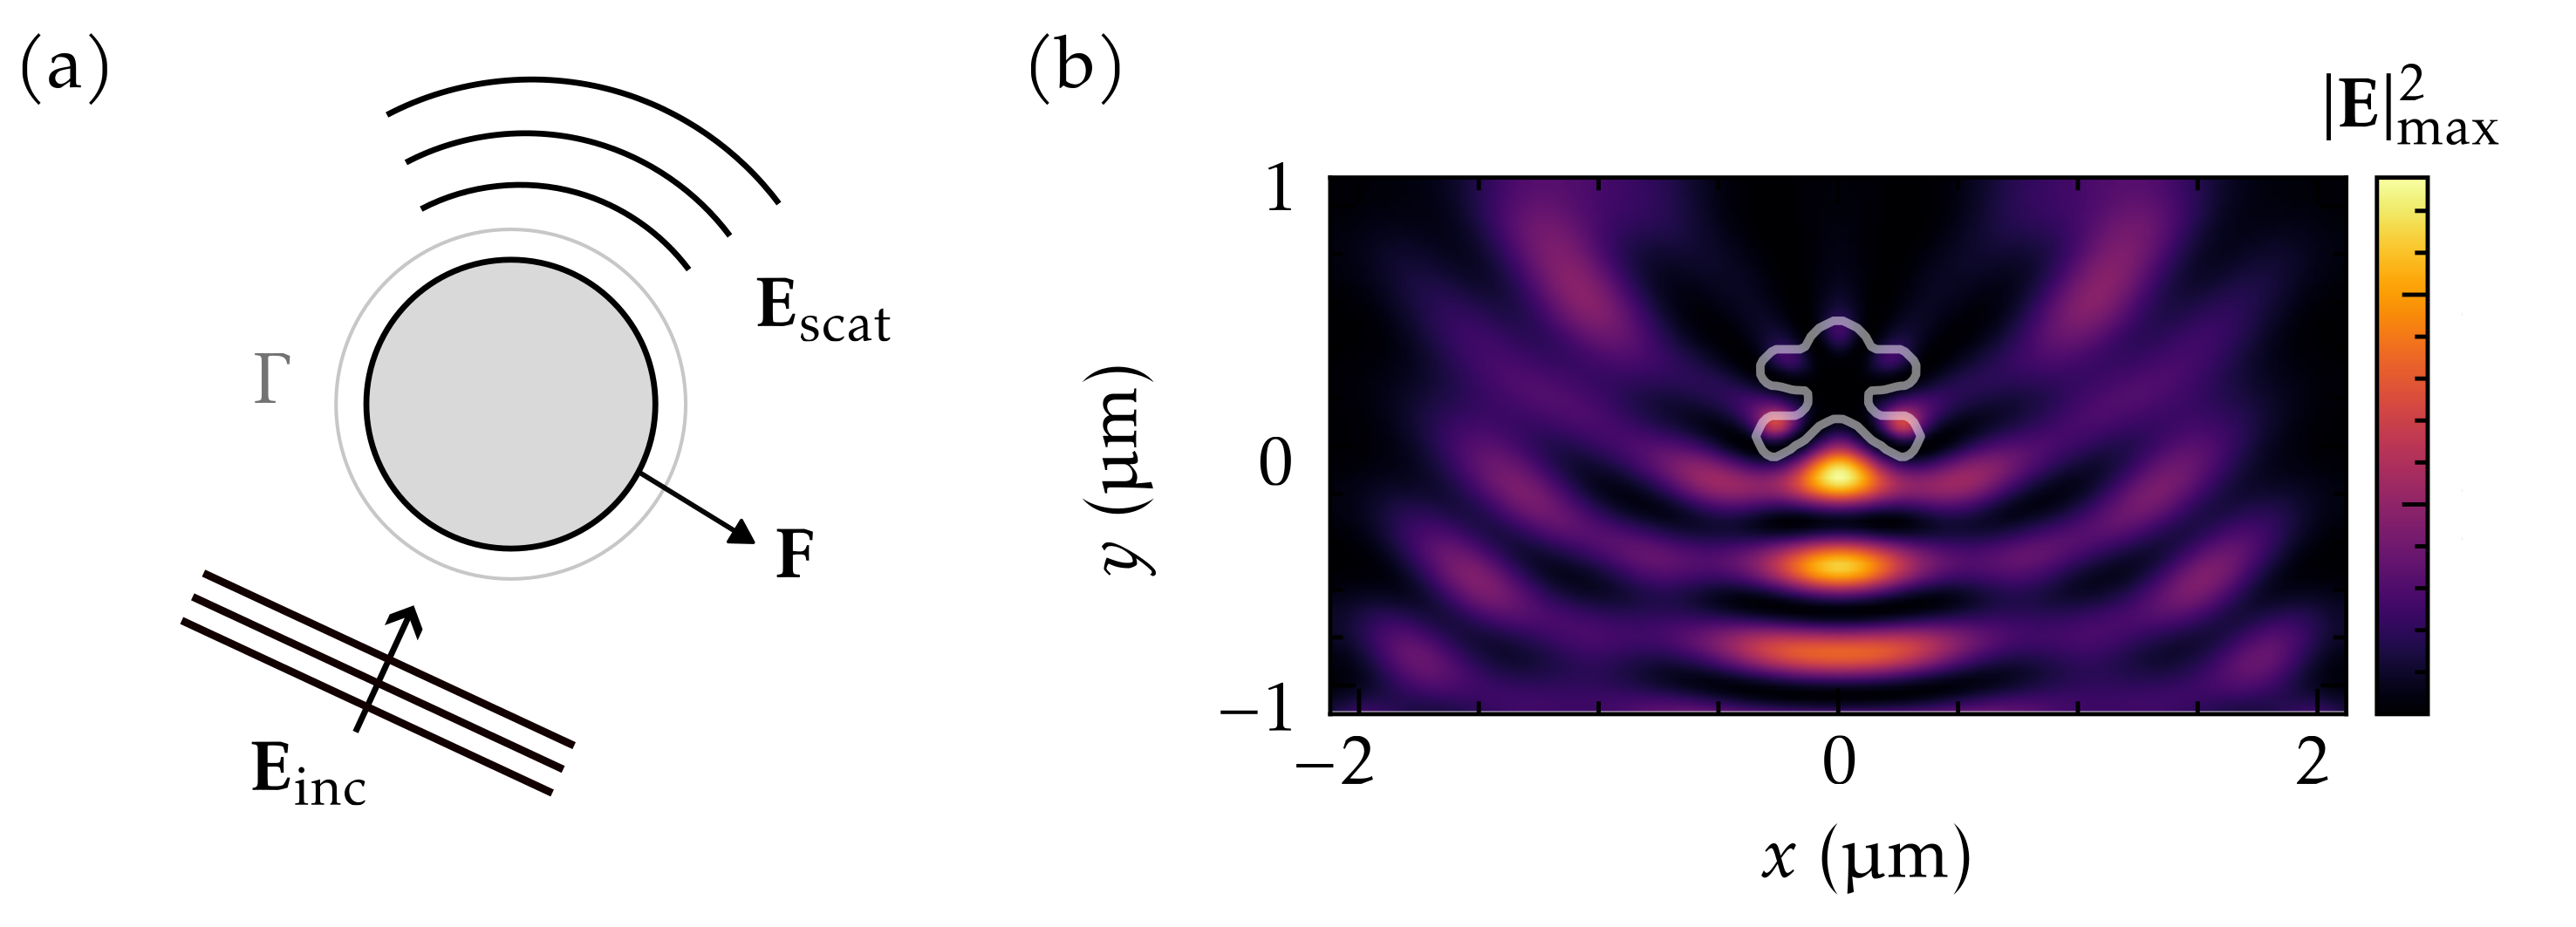
\includegraphics{figures/eng_results.png}}%%
    \caption{Topology optimization in optical force applications. (a) A scattering particle 
    enclosed by a boundary $\partial V$ scatters a field $\mathbf{E}_\text{scat}$, when excited by an incident field $\mathbf{E}_\text{inc}$, 
    generating a net optical force $\mathbf{F}$. (b) Electric-field intensity distribution for a particle design optimized to maximize the vertical ($y$)
    component of the optical force. Adapted with permission from~\cite{ownpub2} \copyright Optical Society of America.}
    \label{fig:eng_res}
\end{figure}

In~\cite{ownpub3} we use this formalism to optimize the geometry of particle-metalens pairs for difference applications, such as attracting, repelling, 
oscillating and trapping particles. In \figref{fig:eng_res} we depict an example optimization result from our work, where 
we optimize the geometry of a particle to maximize the vertical component of the optical force by maximizing $\text{FOM} = \langle\bm{\mathcal{F}}\rangle \cdot \mathbf{n}_y$, where
in our two-dimensional example $\mathbf{n}_y = (0, 1)$ is the unitary vector in the vertical direction.  Our results show that the optimized particle geometry is a Bragg-mirror-like
structure, which is able to efficiently reflecting the incoming plane-wave, resulting in a efficient exchange of force and momentum. In the remainder of~\cite{ownpub3} we extend this example by also designign a metalens to focus the incoming plane-wave onto the particle,
we design attractive particle geometries, and optical-tweezer like setups to trap the particle in space. All the code developed in this work is available on GitHub~\cite{github_MST} with examples on force calculation and topology optimization. 

One interesting aspect of the topology optimization of particles in the MST formalism is that with our current framework the particle cannot feature disconnected members; otherwise
one would need to integrate around the individual components to calculate the total force for each one. It is possible to get around this by enforcing 
a connectivity constraint via the VTM~\cite{li_structural_2016}(see \secref{sec:thermo_optical}). In our examples
we enforce particle connectivity to the center of the design domain, and also of the metalens structure to the bottom, as to ensure Structural
integrity of the structure.

This optimization work is the first, to our knowledge, to 
consider the MST formalism, paving the way for future work in three-dimensional systems and more complex optimization problems, such as optically-driven particle
trajectory control~\cite{zemanek_perspective_2019, macdonald_microfluidic_2003, shilkin_directional_2017}, many-body particle systems~\cite{bechinger_active_2016, chang_colloquium_2018} or optically actuated devices~\cite{ivanyi_optically_2024}, among others.
Finally, it is worth noting that a particularly interesting and straightforward extension would be to use the MST formalism to calculate the time-averaged torque acting on a particle, defined as~\cite{novotny}
\begin{equation}
    \langle \bm{\tau} \rangle = \langle \mathbf{r} \times \bm{\mathcal{F}} \rangle = \int_{\partial V} \langle \mathbf{r}
     \times \stackrel{\leftrightarrow}{\bm{\mathcal{T}}} \rangle \cdot \mathbf{n}_{\partial V} \d\mathbf{r} 
\end{equation}
where $\mathbf{r}$ is the vector defimed between the rotation axis and force application point. This definition of torque accounts
for two kinds of rotational motion; \textit{spinning} ($\langle \bm{\tau}_S \rangle$), where the particle rotates around its center of mass,
and \textit{orbiting} ($\langle \bm{\tau}_O \rangle$), where the particle rotates around an external axis, so that the total torque is the sum
of both the spin and orbital torque $\langle \bm{\tau} \rangle = \langle \bm{\tau}_S \rangle + \langle \bm{\tau}_O \rangle$~\cite{torque}.  Defining
and optical torque-based FOM could open the door for the design of efficient optical and biological micro- and nanomachines~\cite{rotating}.

\subsection*{Optical forces in the dipole approximation~\cite{ownpub1, ownpub3}}

When particles are much smaller than the wavelength of the electromagnetic field ($s\ll \lambda$), it is possible to model the optical force via the dipole approximation in the
quasistatic limit. In this approximation, the particle is treated as a point dipole with a polarizability $\alpha$, which describes how the particle responds to the local electric field frequency-domain $\mathbf{E}$.
In the dipole approximation the optical force on the particle can be expressed as~\cite{novotny}:
\begin{equation}
    \langle\mathbf{F}\rangle=\overbrace{\frac{\alpha^{\prime}}{4} \nabla\left\{\mathbf{E}^* \cdot \mathbf{E}\right\}}^{(1)}
    +\frac{\alpha^{\prime \prime}}{k \varepsilon_0} \Big[\overbrace{\frac{1}{c}\langle \mathbf{S} \rangle}^{(2)} + \overbrace{c \left( \nabla \times \langle \mathbf{L} \rangle \right)}^{(3)}\Big]\,,
\end{equation}
where the polarizability can be split up into the real and imaginary parts 
$\alpha=\alpha^\prime + i \alpha^{\prime \prime}$, the Poynting vector is given by $\mathbf{S} = \mathbf{E} \times \mathbf{H}$, and the time-averaged angular momentum is 
$\langle \mathbf{L} \rangle = [\varepsilon_0/(4 i \omega)](\mathbf{E} \times \mathbf{E}^*)$. 
The term associated with the Poynting vector is the radiation pressure ($2$), while the term associated 
with the angular momentum ($3$) is the spin-curl force.

In the abscence of absorption effects ($\alpha^{\prime \prime}=0$), the force is totally described 
by the gradient force ($1$), which is a conservative force that can be described as the gradient 
of a trapping potential:
\begin{equation*}
    U (\mathbf{r}) = -\frac{\alpha^{\prime}}{4} \left|\mathbf{E}(\mathbf{r})\right|^2\,.
\end{equation*}
where the force can be calculated as $\mathbf{F} = -\nabla U(\mathbf{r})$. 
For non-resonant and non-absorbing isotropic particles the polarizability is 
described through the relation~\cite{BornWolf:1999:Book}
\begin{equation}
    \alpha^{\prime}= 3 \varepsilon_0 $V$ \frac{\varepsilon_p-\varepsilon_m}{\varepsilon_p+2 \varepsilon_m}\,,
\end{equation}
where $V$ is the volume of the particle, $\varepsilon_p$ and $\varepsilon_m$ are the
dielectric constants of the particle and the medium, respectively. Note that in the dipole approximation do not consider the particle modifying
the optical field, which works well for point-like particles in free-space but not necessarily 
for either large particles, particles with high refractive contrast, or particles close to material
boundaries (e.g., optical cavities). This interaction can be accounted for in the dipole
approximation by considering the self-induced back-action (SIBA) effect, which assumes a weak
perturbation of the field due to the particle and expands the field in terms of 
the scattering Green function of the particle, which leads to a self-consistent
equation for the total electric field which can be used to calculate the force~\cite{novotny, SIBA, benjamin}. If the series converges this leads 
to same result as the MST calculation (\eqref{eq:f_MST}), which is often used to validate the dipole approximation (e.g. \cite{ownpub1,ownpub3}). 


Using the dipole approximation formalism in~\cite{ownpub1} we use topology optimization to design an integrated omnidirectional optical trapping chip, which is able to trap particles in three dimensions,
which was previously only possible with the use of free-space optical tweezers~\cite{ashkin_acceleration_1970}, or bulky photonic devices~\cite{manka_simulation_2024}. This is done by minimizing 
the difference of the electric-field norm with respect to a reference field $\mathbf{E}_\text{ref}$:
\begin{equation}
    \text{FOM} \equiv \Phi=\sqrt{\int_{\Omega}\left[\Theta\left(\frac{|\mathbf{E}(\mathbf{r})|}{\left|\mathbf{E}\left(\mathbf{r}_0\right)\right|}-\frac{\left|\mathbf{E}_{\text{ref}}(\mathbf{r})\right|}{\left|\mathbf{E}_{\text{ref}}\left(\mathbf{r}_0\right)\right|}\right)\right]^2} \text{~d} \Omega
    \end{equation}
where the fields are normalized with respect to the value at the center of the design domain $\mathbf{r}_0$, and $\Theta$ is the smoothed Heaviside threshold, which ensures
potentials as steep or steeper than the reference. The reference is chosen as a Gaussian trapping potential, but can be any other potential, such as a harmonic potential ($U\propto\mathbf{r}^2$).

By applying this optimization framework we obtain the topology-optimized cavity design in \figref{fig:MST_dipole}, which is able to trap particles at the center of an optical
cavity in three dimensions and has an associated Gaussian-like trapping potential, with a depth  $U<-10\, k_B T$ at room temperature ($T=300$ K) conventionally needed to overcome Brownian fluctuations~\cite{novotny}.
As long as the dipole approximation is valid one can tune the input power to trap paricles of arbitrarily small sizes.

\begin{figure}[tb]
    \centering
    \makebox[\textwidth][c]{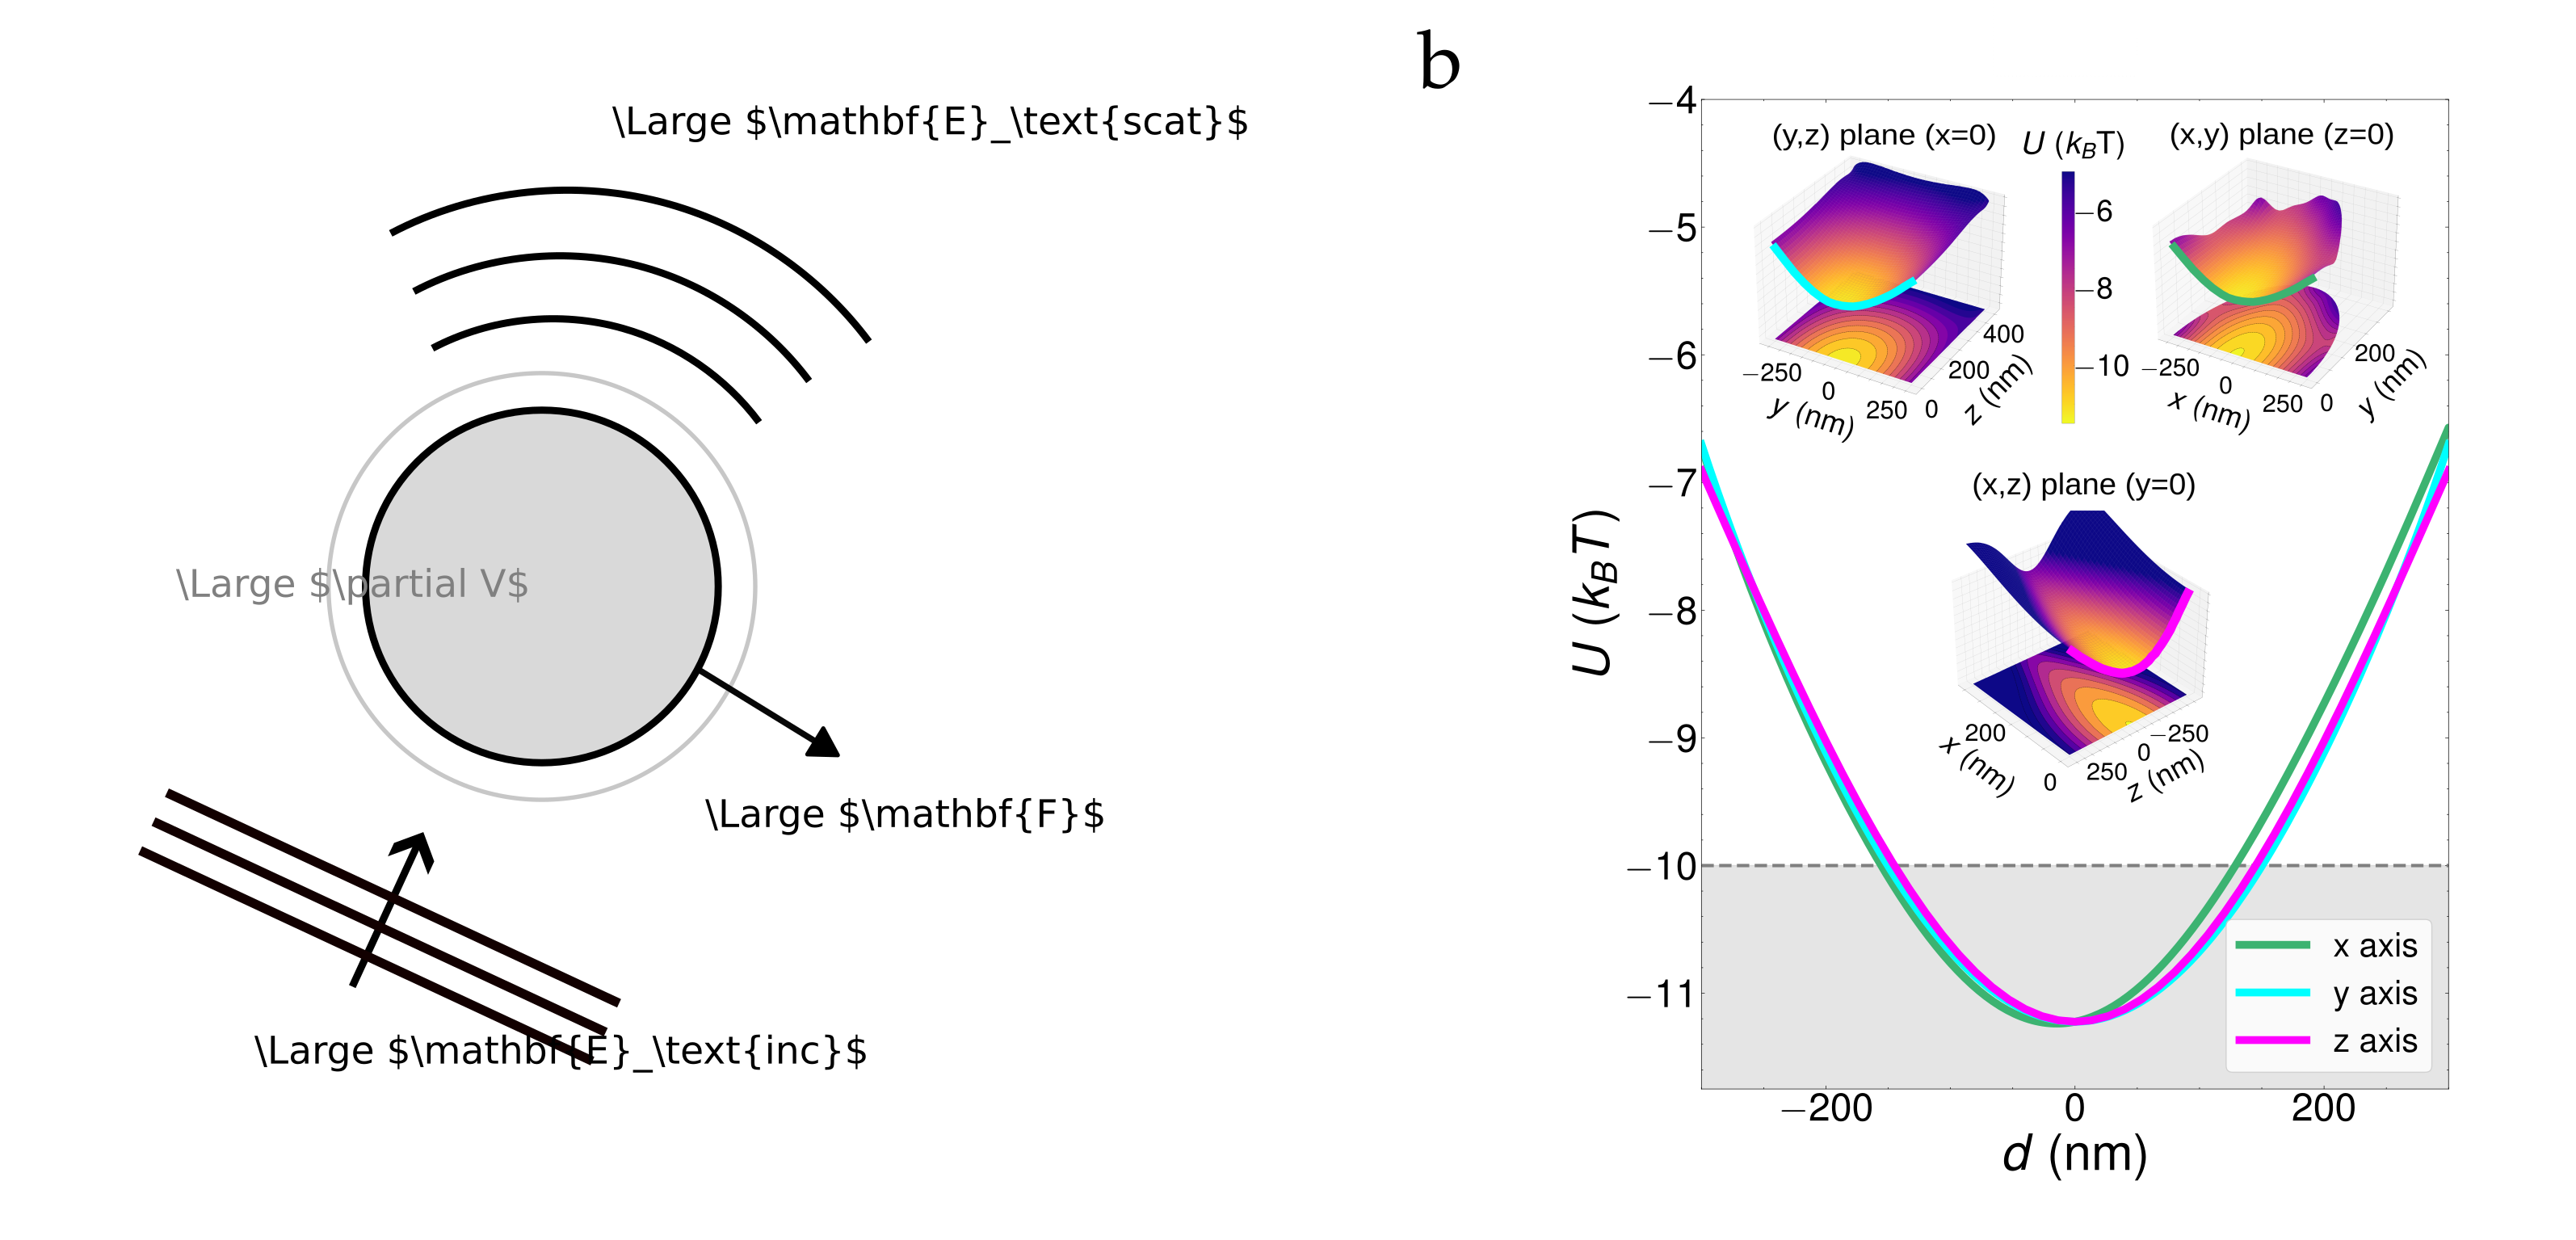
\includegraphics{figures/MST_dipole.png}}%%
    \caption{Optical response and trappig potential for the topology-optimized particle trap. (a) Lower half ($z<0$) of the optimized cavity, with the electric-field intensity
    distribution when excited with the fundamental waveguide mode at $\lambda=1.55$ \textmu m. (b) Trapping potential for a $R=15$ nm and $n=2$ particle in the cavity region for the different axial line- and plane-cuts as a function
    of the distance from the center ($d$), with the stable trapping regime ($U<-10 k_B\, T$) highlighted in gray. Adapted with permission from~\cite{ownpub1}.}
    \label{fig:MST_dipole}
\end{figure}

From the dipole approximation trapping potential we calculate the the force-displacements curves and we determine trapping stiffnesses
of $\kappa \approx 0.5$ fN/nm, an order of magnitude larger that diffraction-limited free-space optical tweezers~\cite{ownpub1}. To validate this findings
we employ the MST formalism to calculating the force on spherical particles as they are displaced from the cavity center in the axial directions, and find excellent
agreement with the dipole approximation. As shown in \figref{fig:SPIE}, to further verify the the dipole approximation assumption in ~\cite{ownpub3} we compare the results of the dipole approximation with the MST
for varying particle sizes and refractive indices, showing that the dipole approximation is a good approximation
even for large values of the refractive index (e.g., $n=3$) and particle sizes up to $s\approx 0.05 \lambda$. As we can see for larger sizes and refractive indices 
the results start to deviate, and the dipole approximation should break down for even larger values.

\begin{figure}[tb]
    \centering
    \makebox[\textwidth][c]{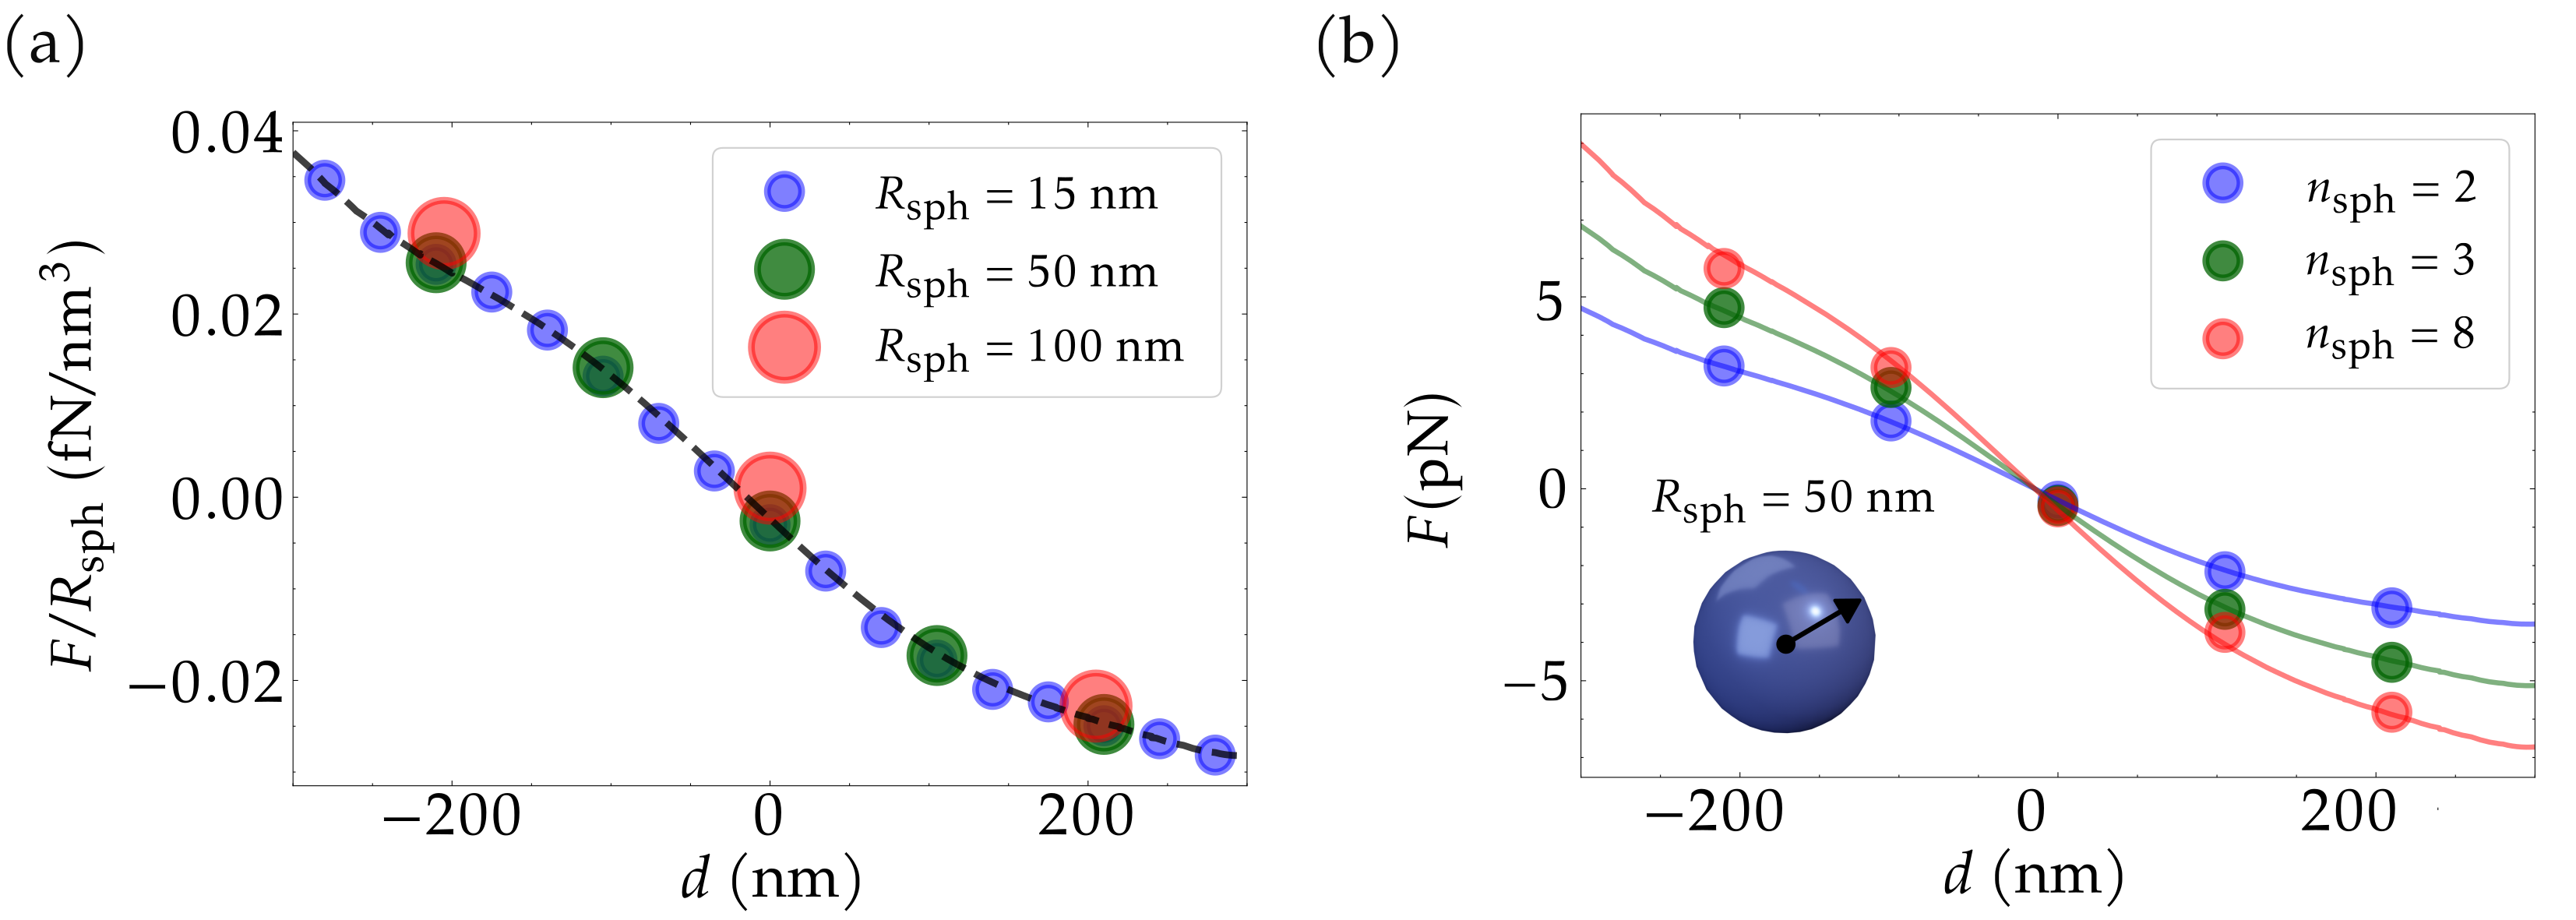
\includegraphics{figures/SPIE_results.png}}%%
    \caption{Validating the dipole approximation force (dashed line) against the MST force (data points), for the force as a function of displacement ($d$) from the cavity center.
    (a) Volume-normalized force ($F/R^2_\text{sph}$) for different particle sizes with refractive index $n_\text{sph}=2$. (b) Force for different refractive indices of the particle for a particle radius $R_\text{sph}=50$ nm. Adapted from~\cite{ownpub3}.}
    \label{fig:SPIE}
\end{figure}

When designing optical trapping platforms it is important to be able to compare performance across platforms. To this end, in~\cite{ownpub3} we introduce a normalized
trapping stiffness metric, which normalizes trapping stiffness to particle  polarizability and input power ($P_\text{in}$)
\begin{equation}
    \eta_i=\frac{\kappa_i \varepsilon_0}{\alpha^\prime P_{\text{in}}}
\end{equation}
enabling one-to-one comparison across trapping devices\footnote{As noted in~\cite{ownpub3} this metrics breaks down for lightless platforms (e.g. Casimir force-based traps), and the metric could be redefined
without including the input power.}. The normalized trapping stiffness allows us to show that (Tab. 1 in~\cite{ownpub3}), although plasmonic devices can reach higher normalized 
stiffnesses, they suffer from optical losses to heating and lack omnidirectional stability. In contrast, our inverse-designed dielectric platform
 achieves comparable normalized stiffnesses to other dielectric traps while uniquely offering fully stable, omnidirectional trapping
  without relying on SIBA effects. Notably, SIBA-based devices are particle-specific and their performance can break down
   for different particle geometries or materials. Compared to conventional optical tweezers, our device maintains similar trapping
    strength at lower input power due to its integrated, waveguide-coupled design, highlighting the benefits of miniaturized,
     near-field-based optical trapping.

Lastly, in~\cite{ownpub2} we also discuss the effects of Casimir Polder effects on particle loading into the trap, and
also discuss possible applications of our proposed devices in particle optomechanics and
biophotonics, where the ability to control a trapped particle omnidirectionally in a compact integrated device
couled lead to novel technological applications.

\subsection*{Strongly coupled optomechanical systems}

Mechanical steady-state force balance
\begin{equation}
    \nabla \cdot \overleftrightarrow{\boldsymbol{\sigma}} + \mathbf{f} = 0\,,
\end{equation}
Stress tensor:
\begin{equation}
    \nabla \cdot \overleftrightarrow{\boldsymbol{\sigma}} + \nabla \cdot \overleftrightarrow{\mathbf{T}} = 0\,,
\end{equation}

In strongly coupled optomechanical systems, the optical field can significantly modify the mechanical properties of the system, leading to a significant deformation
of the device, which in turn modifies the optical response. 

We have studied these systems in terms of topology optimization, as part of some unpublished work. In this work we consider 
the mechanical deformation of a membrane-like system, which is optically excited by a plane-wave. The optical field is calculated using the MST,
and the mechanical deformation is calculated using the linear elasticity theory. The mechanical deformation is then used to modify the optical field, 
leading to a self-consistent problem that can be solved iteratively, similar to other work.

ADD SOME OF THE WORK WITH THE MEMBRANE-LIKE SYSTEM HERE. TO BE FINISHED!


\section{Electro-optical systems~\cite{ownpub4}}

Electro-optics describes the interaction between external electricity and optics, where the frquency of the electrical fields ($\omega_E$)
have much lower frequencies than the optical fields ($\omega_E \ll \omega $), so that they can be considered as static fields.
This coupling is used in a variety of technologies such as high-speed modulators for optical communications, 
tunable filters and switches, adaptive optics, electrically pumped lasers, and integrated photonic circuits. 
These systems exploit mechanisms ranging from direct electro-optic modulation to carrier-induced refractive index
 changes and electro-optic control inside laser cavities for pulse shaping and frequency tuning. ADD CITATION USE POCKELS AND CHANGE
 APPLICATIONS.

As an example of electro-optic coupling one can consider the electro-optic effect (analogous to the thermo-optic effect),
where the refractive index of a material can be modified by applying an external electric field, where the linear term is known as the
Pockels effect~\cite{pockels} $
    \Delta n = -(1/2) n^3 r E\,,$
where $r$ is the electro-optic coefficient, and $E$ is the applied electric field. The quadratic term 
is known as the electro-optic Kerr effect where $\Delta n = n_2 E^2$, where $n_2$ is the Kerr-coefficient~\cite{phot_crys}. Note that by considering an external
quasistatic electric field, one can model the nonlinearities by accounting for higher order terms in the expansion of the polarizability
in terms of the electric field (\eqref{eq:polarization}), where the Pockels effect corrresponds to the $\chi^{(2)}$ term, and the Kerr effect to the $\chi^{(3)}$ term.

Topology optimization has been used been extensively used to study coupled electrical systems
such as, MEMS devices~\cite{MEMS_multi}, electrochemical systems~\cite{electrode}, and electrostatic actuators~\cite{electrostatic_act}. However, the field of electro-optics is
still relatively unexplored with few works, such as \cite{g_heat}, which studies the design of diffusion-based systems with applications on
carrier dynamics in semiconductor devices.

In the remainder of the section we focus on our work~\cite{ownpub4} , which harness electro-optics 
to achieve efficient light emission through electrical pumping.

\subsection*{Topology optimization of nanolasers~\cite{ownpub4}}

A nanolaser is a nanoscale laser device that emits light by stimulating the emission of photons in a gain medium, typically a semiconductor material. This is illustrated
in \figref{fig:laser2d}, where a pump laser excites the emitters (e.g. carriers) in a gain medium $D_0$, which then emits light into an output channel (e.g. waveguide). This physical
mechanism can be described by using thre Maxwell-Bloch equations~\cite{haken_laser_dynamics, PhysRev.134.A1429, SALT_original}, which are a set of nonlinear time-dependent 
partial differential equations that relate the electric field, the polarization and the population inversion ($D$). Nevertheless, when aligned to high-$Q$ ($Q\gtrapprox 100$~\cite{cerjan_2016}) single-mode semiconductor laser
mode, the system can be described via the single-pole approximation (SPA-) steady-state ab-initio laser theory (SALT)~\cite{Ge_2010}
\begin{equation}\label{eq:SPA_SALT}
    {\left[(\nabla \times 
     \nabla \times ) -\left(\varepsilon_c(\mathbf{r})-i \Delta \varepsilon_\Im (\mathbf{r})\right) \left(\frac{\omega_L}{c}\right)^2\right] \mathbf{E}_L(\mathbf{r})=0}\,.
\end{equation}
where $\mathbf{E}_L$ is the lasing mode, $\omega_L$ is the lasing frequency, $\varepsilon_c$ is the bare dielectric permittivity (without gain), and the change in the 
imaginary part of the permittivity is given by
where the change in the dielectric permittivity is given by
\begin{equation}\label{eq:gain_SALT}
        \Delta \varepsilon_\Im (\mathbf{r}) =  \frac{D_0(\mathbf{r}) d}{1+ e_c^{-2}\left|\mathbf{E}_L(\mathbf{r})\right|^2}\,.
\end{equation}
where $D_0(\mathbf{r})$ is the gain profile, $d$ is a scalar pumping strength, $e_c$ is a non-dimensionalization parameter~\cite{Ge_2010}. Although much simpler than the Maxwell-Bloch equations, \eqref{eq:SPA_SALT} still
requires one to solve a nonlinear eigenproblem, which is more complex an more computationally expensive than solving a linear system.

\begin{figure}[tb]
    \centering
    \makebox[\textwidth][c]{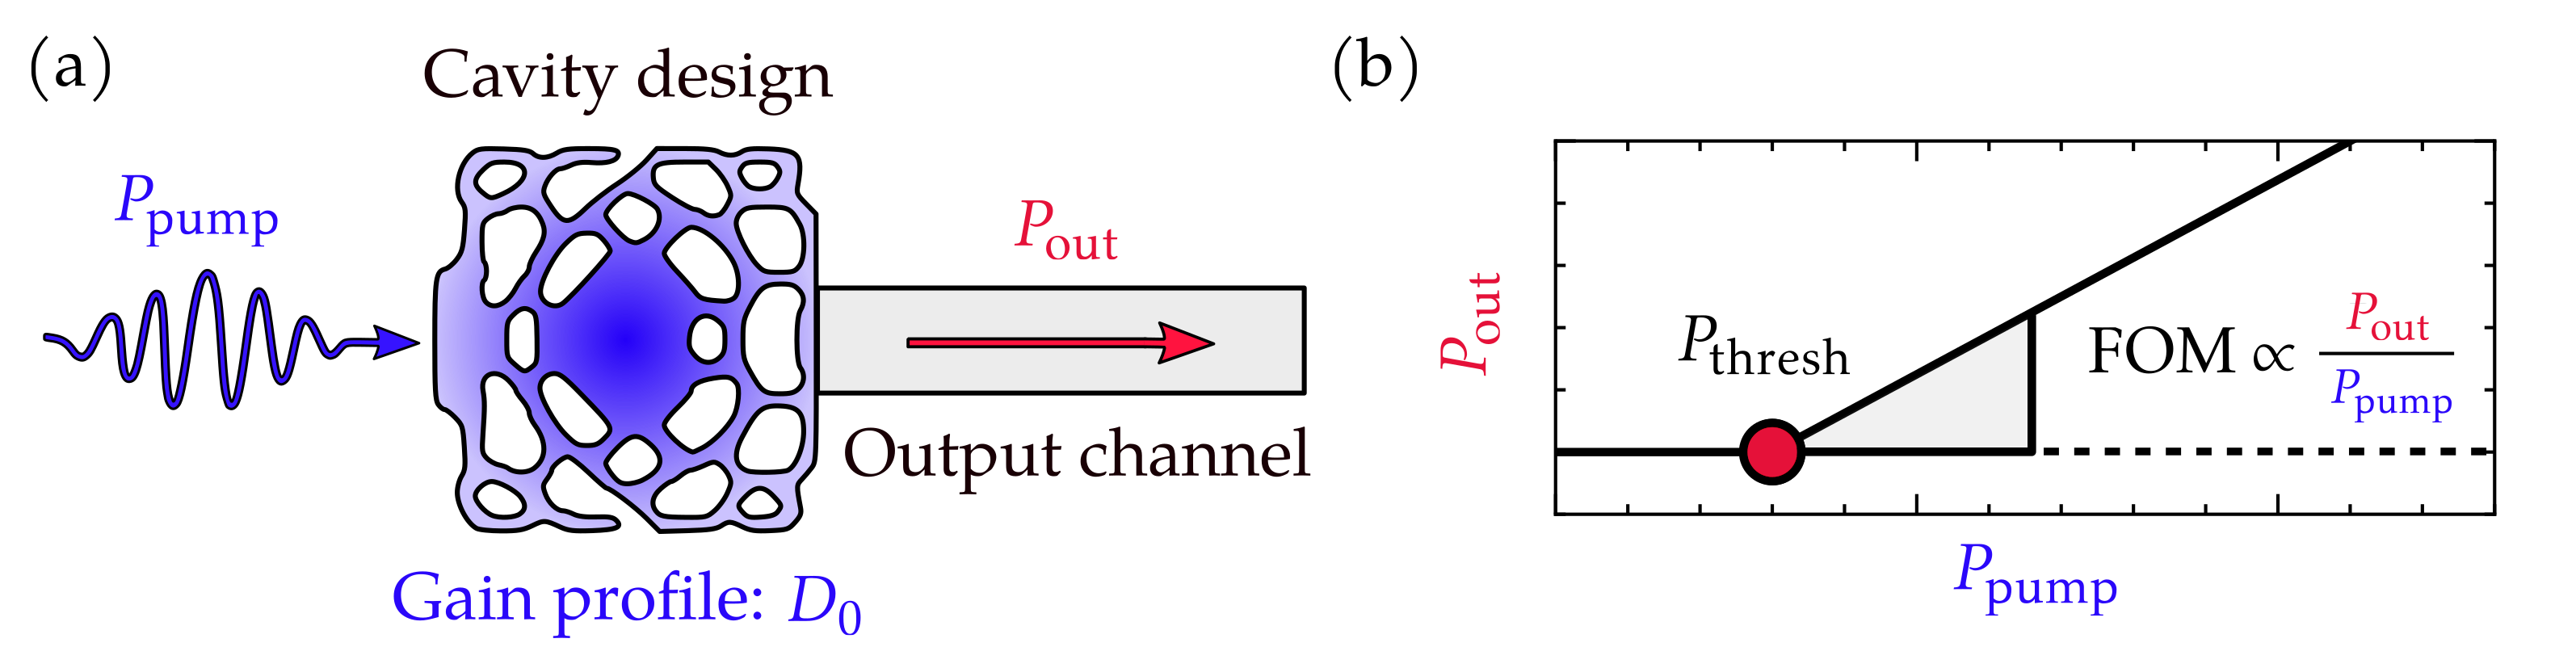
\includegraphics{figures/laser.png}}%%
    \caption{Topology optimization of nanolasers. (a) Working principle of a nanolaser. A pump power ($P_\text{pump}$) excites a a gain medium with profile
    $D_0$ that emits a single lasing mode into an output channel with power $P_\text{out}$. (b) The optimization FOM considers the linear relation between the pump and output power ($P_\text{out}/P_\text{pump}$),
    just above the lasing threshold ($P \gtrapprox P_\text{thres}$). (c) Topology optimization with carrier diffusion effects, where the gain profile $D_0$ is diffused ($\mathbb{S}[D_0]$)
    in the semiconductor-like material. Adapted from~\cite{ownpub4}. MAKE RIGHT PLOT LARGER AND ADJUST THE REST, B SHOULD BE TALLER AND A SHOULD BE SCALED DOWN. FOM SHOULD NOT BE EQUAL.}
    \label{fig:laser2d}
\end{figure}

To circumvent this in~\cite{ownpub4} we use a synthesis of SPA-SALT, perturbation theory, coupled mode theory to simplify the problem to a linear system of equations. 
A key result is the calculation of the lasing threshold~\cite{ownpub4}
\begin{equation}\label{eq:pump_thresh}
    d_\text{thresh} = \frac{\Gamma}{Q} = \frac{1}{Q} \frac{\int_{\Omega} \varepsilon_c(\mathbf{r})|\mathbf{E}_{\text{m}}(\mathbf{r})|^2\,  \d \Omega}{\int_{\Omega} D_0(\mathbf{r}) |\mathbf{E}_{\text{m}}(\mathbf{r})|^2\,  \d \Omega}\,.
\end{equation}
where $\mathbf{E}_\text{m}$ is the passive cavity mode. From this expression we see that one can reduce the lasing threshold (for more energy-efficient lasers) by increasing $Q$ and decreasing $\Gamma$ by enhancing the energy confinement in the
active medium. Note that in the limit of a single-emitter limit, where $D_0(\mathbf{r})\propto \delta (\mathbf{r}-\mathbf{r^\prime})$ for an emitter located at $\mathbf{r}^\prime$, this expression becomes $d_\text{thresh}=V/Q$, where $V$ is a measure
of the modal volume.

The main result of the work is a FOM that can be evaluated by solving a reciprocal problem where the system is excited from then output port~\cite{ownpub4}
\begin{equation}\label{eq:eff_nl}
    \frac{P_\text{out}}{P_\text{pump}} \propto \frac{\left( \int_{\Omega} D_0(\mathbf{r})|\mathbf{E}_{\text{r}}(\mathbf{r})|^2 \,  \d \Omega \right)^3} {\int_{\Omega} D_0(\mathbf{r}) |\mathbf{E}_{\text{r}}(\mathbf{r})|^4 \,  \d \Omega} = \text{FOM}.
\end{equation}
where $\mathbf{E}_{\text{r}}$ is the field distribution in the reciprocal problem. The FOM is a metric proportional to the laser efficiency ($P_\text{out}/P_\text{pump}$), and is roughly proportional 
to the energy in the cavity ($\sim |\mathbf{E}_{\text{r}}|^6 / |\mathbf{E}_{\text{r}}|^4 \sim |\mathbf{E}_{\text{r}}|^2$), and thus to the $Q$ factor, also contributing to a low
laser threshold (\eqref{eq:pump_thresh}). Thefore, as the optimization progresses the high-$Q$ assumption will become more and more accurate. Note that in the single emitter limit the FOM becomes
$\text{FOM}=\int_{\Omega} D_0(\mathbf{r}) |\mathbf{E}_{\text{r}}(\mathbf{r})|^2 \d \Omega$, which via reciprocity is proportional to the total power emitted into an output channel~\cite[App.~C]{reci}. 

In semiconductors with extended media, it is essential to model the electrical proccess of carrier diffusion. This effect can be introduced by modeling the semiconductor gain medium in the free-carrier approximation\footnote{Neglecting carrier-carrier Coulomb interactions.}, using a difussion 
equation\cite{csalt}. Using this formalism we derive the same expressions when accounting for carrier diffusion~\cite{ownpub4}, where the lasing threshold is
\begin{equation}\label{eq:pump_thresh_diff}
    d_\text{thresh} = \frac{1}{Q} \frac{\int_{\Omega} \varepsilon_c(\mathbf{r})|\mathbf{E}_{\text{m}}(\mathbf{r})|^2\,  \d \Omega}{\int_{\Omega} \mathbb{S} [D_0] (\mathbf{r}) |\mathbf{E}_{\text{m}}(\mathbf{r})|^2\,  \d \Omega}\,,
\end{equation}
and the FOM is given by
\begin{equation}\label{eq:eff_diff}
    \text{FOM} \propto  \frac{\left(\int_{\Omega} \mathbb{S} [D_0](\mathbf{r}) |\mathbf{E}_{\text{r}}(\mathbf{r})|^2 \,  \d \Omega\right)^3} {\int_{\Omega} \mathbb{S}\left[ |\mathbf{E}_{\text{r}}|^2\, \mathbb{S} [D_0] \right] (\mathbf{r})|\mathbf{E}_{\text{r}}(\mathbf{r})|^2 \,  \d \Omega}\,.
\end{equation}
These expressions use the diffusion operator $\mathbb{S}^{-1}= \mathbb{I}+\nabla \cdot (R_\nabla^2(\mathbf{r}) \nabla)$, where $\mathbb{I}$ is the identity operator, and $R_\nabla (\mathbf{r})$ is a diffusion lengthscale determined by the spatially- and design-dependent diffusion coefficient combined with the damping/recombination rate. 
In this notation computing $u = \mathbb{S}[b]$ corresponds to solving for the scalar field $u$ in the diffusion problem $\mathbb{S}^{-1}u=b$, where $b$ is a scalar field. 
The difference when accounting for difussion is that now one needs to consider the profile of diffused carriers $\mathbb{S} [D_0]$ in the lasing threshold, and the diffusion of the gain depletion
in the FOM denominator. Note that in the small diffusion limit ($R_\nabla \ll \lambda, \mathbb{S} \approx \mathbb{I}$)
we recover the original expressions in \eqref{eq:pump_thresh} and \eqref{eq:eff_nl}.

Using this new formulation for nanolaser optimization we optimize nanolaser devices in two and three dimensions. In two dimensions we study the effect of the gain region size in 
nanolaser design, and verify that for point-like gain regions the derived FOM and an LDOS-like FOM become equivalent. Moreover, we show that for
larger distributed gain media the derived FOM discourages field localization, in contrast to the LDOS-like metric. We also see how accounting for diffusion effects
affects nanolaser designs, as shown in \figref{fig:laser2d}, the device that accounts for diffusion disconnects the cavity from the waveguide, to 
enhance the coupling between the carriers and the optical field. Finally, we also apply the formalism to design three-dimensional silicon-on-insulator nanolasers (\figref{fig:laser3d}), 
and verify that similar to the two-dimensional case, the FOM discourages field localization while still efficiently coupling to the output waveguide.

\begin{figure}[tb]
    \centering
    \makebox[\textwidth][c]{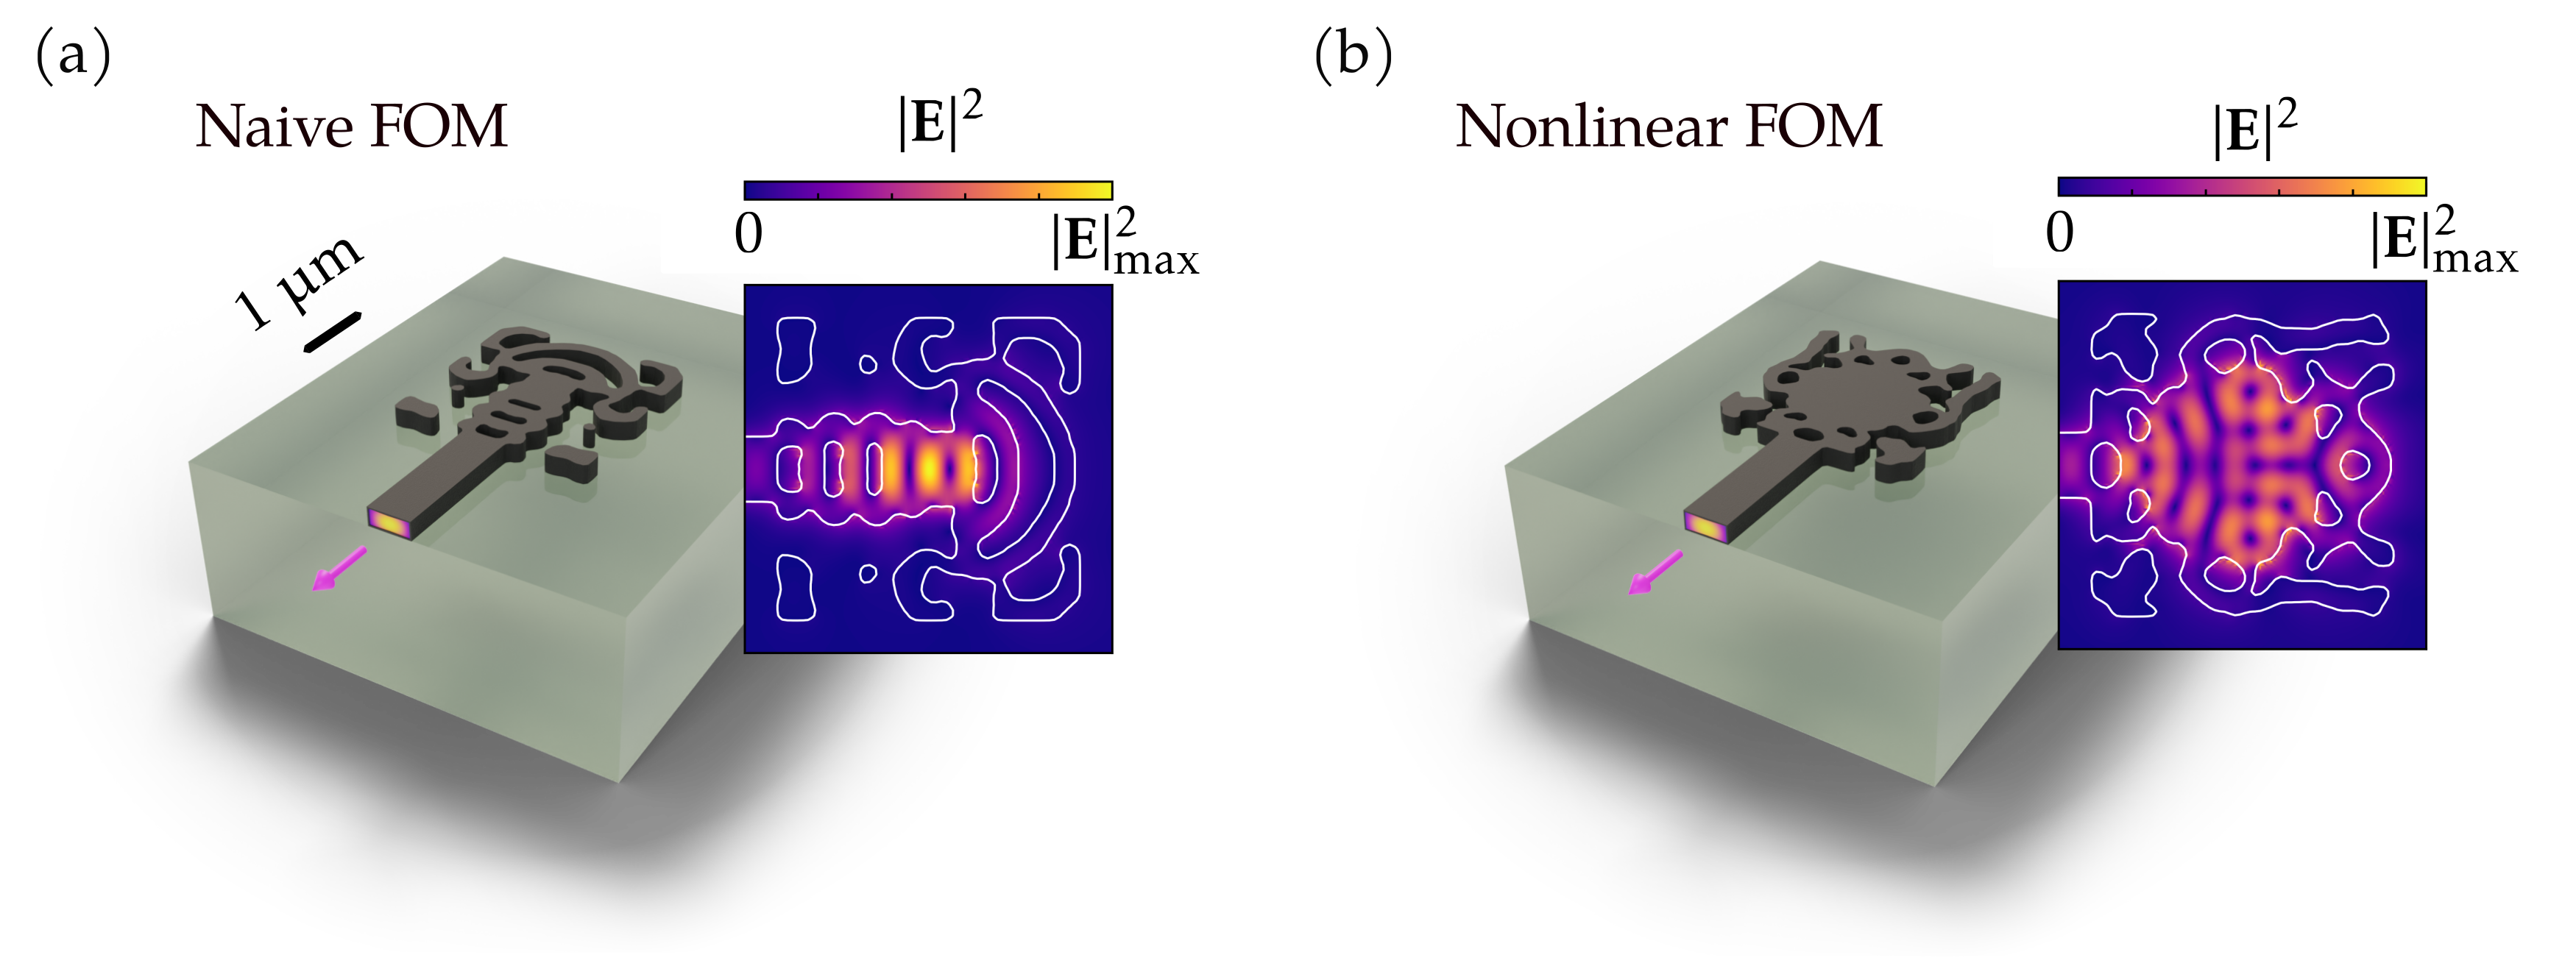
\includegraphics{figures/laser_2.png}}%%
    \caption{Topology-optimized nanolasers in three dimensions. The devices las into the cavity mode (inset plot) and out-couple to the
    mostly-$H_z$ waveguide mode. (a) Device optimized for the naive FOM. (b) Device optimized for the nonlinear FOM.}
    \label{fig:laser3d}
\end{figure}
